%*******************************************************************************
% Name : PAPD - PART ASSOCIATION FOR PEDESTRIAN DETECTION
% Author : HAANJU.YOO
% Initial Date : 2015.10.19 (originally for CVPR)
% Last Update : ____.__.__
% Version : 0.9
%*******************************************************************************
%                                            ....
%                                           W$$$$$u
%                                           $$$$F**+           .oW$$$eu
%                                           ..ueeeWeeo..      e$$$$$$$$$
%                                       .eW$$$$$$$$$$$$$$$b- d$$$$$$$$$$W
%                           ,,,,,,,uee$$$$$$$$$$$$$$$$$$$$$ H$$$$$$$$$$$~
%                        :eoC$$$$$$$$$$$C""?$$$$$$$$$$$$$$$ T$$$$$$$$$$"
%                         $$$*$$$$$$$$$$$$$e "$$$$$$$$$$$$$$i$$$$$$$$F"
%                         ?f"!?$$$$$$$$$$$$$$ud$$$$$$$$$$$$$$$$$$$$*Co
%                         $   o$$$$$$$$$$$$$$$$$$$$$$$$$$$$$$$$$$$$$$$$
%                 !!!!m.*eeeW$$$$$$$$$$$f?$$$$$$$$$$$$$$$$$$$$$$$$$$$$$U
%                 !!!!!! !$$$$$$$$$$$$$$  T$$$$$$$$$$$$$$$$$$$$$$$$$$$$$
%                  *!!*.o$$$$$$$$$$$$$$$e,d$$$$$$$$$$$$$$$$$$$$$$$$$$$$$:
%                 "eee$$$$$$$$$$$$$$$$$$$$$$$$$$$$$$$$$$$$$$$$$$$$$$$$$$C
%                b ?$$$$$$$$$$$$$$**$$$$$$$$$$$$$$$$$$$$$$$$$$$$$$$$$$$$!
%                Tb "$$$$$$$$$$$$$$*uL"$$$$$$$$$$$$$$$$$$$$$$$$$$$$$$$$$'
%                 $$o."?$$$$$$$$F" u$$$$$$$$$$$$$$$$$$$$$$$$$$$$$$$$$$$$
%                  $$$$en ```    .e$$$$$$$$$$$$$$$$$$$$$$$$$$$$$$$$$$$$'
%                   $$$B*  =*"?.e$$$$$$$$$$$$$$$$$$$$$$$$$$$$$$$$$$$$$F
%                    $$$W"$$$$$$$$$$$$$$$$$$$$$$$$$$$$$$$$$$$$$$$$$$$"
%                     "$$$o#$$$$$$$$$$$$$$$$$$$$$$$$$$$$$$$$$$$$$$$$"
%                    R: ?$$$W$$$$$$$$$$$$$$$$$$$$$$$$$$$$$$$$$$$$$" :!i.
%                     !!n.?$???""``.......,``````"""""""""""``   ...+!!!
%                      !* ,+::!!!!!!!!!!!!!!!!!!!!!!!!!!!!!!!!!!!!!!!*`
%                      "!?!!!!!!!!!!!!!!!!!!~ !!!!!!!!!!!!!!!!!!!~`
%                      +!!!!!!!!!!!!!!!!!!!! !!!!!!!!!!!!!!!!!!?!`
%                    .!!!!!!!!!!!!!!!!!!!!!' !!!!!!!!!!!!!!!, !!!!
%                   :!!!!!!!!!!!!!!!!!!!!!!' !!!!!!!!!!!!!!!!! `!!:
%                .+!!!!!!!!!!!!!!!!!!!!!~~!! !!!!!!!!!!!!!!!!!! !!!.
%               :!!!!!!!!!!!!!!!!!!!!!!!!!.`:!!!!!!!!!!!!!!!!!:: `!!+
%               "~!!!!!!!!!!!!!!!!!!!!!!!!!!.~!!!!!!!!!!!!!!!!!!!!.`!!:
%                   ~~!!!!!!!!!!!!!!!!!!!!!!! ;!!!!~` ..eeeeeeo.`+!.!!!!.
%                 :..    `+~!!!!!!!!!!!!!!!!! :!;`.e$$$$$$$$$$$$$u .
%                 $$$$$$beeeu..  `````~+~~~~~" ` !$$$$$$$$$$$$$$$$ $b
%                 $$$$$$$$$$$$$$$$$$$$$UU$U$$$$$ ~$$$$$$$$$$$$$$$$ $$o
%                !$$$$$$$$$$$$$$$$$$$$$$$$$$$$$$. $$$$$$$$$$$$$$$~ $$$u
%                !$$$$$$$$$$$$$$$$$$$$$$$$$$$$$$! $$$$$$$$$$$$$$$ 8$$$$.
%                !$$$$$$$$$$$$$$$$$$$$$$$$$$$$$$X $$$$$$$$$$$$$$`u$$$$$W
%                !$$$$$$$$$$$$$$$$$$$$$$$$$$$$$$! $$$$$$$$$$$$$".$$$$$$$:
%                 $$$$$$$$$$$$$$$$$$$$$$$$$$$$$$  $$$$$$$$$$$$F.$$$$$$$$$
%                 ?$$$$$$$$$$$$$$$$$$$$$$$$$$$$f $$$$$$$$$$$$' $$$$$$$$$$.
%                  $$$$$$$$$$$$$$$$$$$$$$$$$$$$ $$$$$$$$$$$$$  $$$$$$$$$$!
%                  "$$$$$$$$$$$$$$$$$$$$$$$$$$$ ?$$$$$$$$$$$$  $$$$$$$$$$!
%                   "$$$$$$$$$$$$$$$$$$$$$$$$Fib ?$$$$$$$$$$$b ?$$$$$$$$$
%                     "$$$$$$$$$$$$$$$$$$$$"o$$$b."$$$$$$$$$$$  $$$$$$$$'
%                    e. ?$$$$$$$$$$$$$$$$$ d$$$$$$o."?$$$$$$$$H $$$$$$$'
%                   $$$W.`?$$$$$$$$$$$$$$$ $$$$$$$$$e. "??$$$f .$$$$$$'
%                  d$$$$$$o "?$$$$$$$$$$$$ $$$$$$$$$$$$$eeeeee$$$$$$$"
%                  $$$$$$$$$bu "?$$$$$$$$$ 3$$$$$$$$$$$$$$$$$$$$*$$"
%                 d$$$$$$$$$$$$$e. "?$$$$$:`$$$$$$$$$$$$$$$$$$$$8
%         e$$e.   $$$$$$$$$$$$$$$$$$+  "??f "$$$$$$$$$$$$$$$$$$$$c
%        $$$$$$$o $$$$$$$$$$$$$$$F"          `$$$$$$$$$$$$$$$$$$$$b.0
%       M$$$$$$$$U$$$$$$$$$$$$$F"              ?$$$$$$$$$$$$$$$$$$$$$u
%       ?$$$$$$$$$$$$$$$$$$$$F                   "?$$$$$$$$$$$$$$$$$$$$u
%        "$$$$$$$$$$$$$$$$$$"                       ?$$$$$$$$$$$$$$$$$$$$o
%          "?$$$$$$$$$$$$$F                            "?$$$$$$$$$$$$$$$$$$
%             "??$$$$$$$F                                 ""?3$$$$$$$$$$$$F
%                                                       .e$$$$$$$$$$$$$$$$'
%                                                      u$$$$$$$$$$$$$$$$$
%                                                     `$$$$$$$$$$$$$$$$"
%                                                      "$$$$$$$$$$$$F"
%                                                        ""?????""
%
%*******************************************************************************

\documentclass[runningheads]{llncs}
\usepackage{cite}
\usepackage{times}
\usepackage{kotex}
\usepackage{epsfig}
\usepackage{lmodern}
\usepackage{textcomp}
\usepackage{amsmath}
\usepackage{amssymb}
\usepackage{amsfonts}
\usepackage{ruler}
\usepackage{graphicx}
\usepackage{algorithm}
\usepackage{algpseudocode}
\usepackage{multirow}
\usepackage[table,xcdraw]{xcolor}
\usepackage[misc,geometry]{ifsym}
\usepackage[pagebackref=true,breaklinks=true,letterpaper=true,colorlinks,bookmarks=false]{hyperref}
\usepackage[width=122mm,left=12mm,paperwidth=146mm,height=193mm,top=12mm,paperheight=217mm]{geometry}
%==============================================================================
\newcommand{\norm}[1]{\left\lVert#1\right\rVert}
\DeclareMathOperator*{\argmax}{arg\,max}
%==============================================================================

\begin{document}
% \renewcommand\thelinenumber{\color[rgb]{0.2,0.5,0.8}\normalfont\sffamily\scriptsize\arabic{linenumber}\color[rgb]{0,0,0}}
% \renewcommand\makeLineNumber {\hss\thelinenumber\ \hspace{6mm} \rlap{\hskip\textwidth\ \hspace{6.5mm}\thelinenumber}}
% \linenumbers
\pagestyle{headings}
\mainmatter
\def\ECCV16SubNumber{***}  % Insert your submission number here

\title{Part Assignment for Pedestrian Detection \\ in Crowded Scene}

\titlerunning{ECCV-16 submission ID \ECCV16SubNumber}

\authorrunning{ECCV-16 submission ID \ECCV16SubNumber}

\author{Anonymous ECCV submission}
\institute{Paper ID \ECCV16SubNumber}

\maketitle
%==============================================================================

%%%%%%%%%%%%%%%%%%%%%%%%%%%%%%%%%%%%%%%%%%%%%%%%%%%%%%%%%%%%%%%%%%%%%%%%%%%%%%%
% ABSTRACT
%%%%%%%%%%%%%%%%%%%%%%%%%%%%%%%%%%%%%%%%%%%%%%%%%%%%%%%%%%%%%%%%%%%%%%%%%%%%%%%
\begin{abstract}
% 풀고자 하는 문제
  We propose the novel method to detection pedestrians in crowded scenes, and to provide an exact visible appearance of partially occluded pedestrians.
  % 기존의 연구
  Although the state-of-the art detection methods based on a single pedestrian have achieved a great performance on moderate scenes, they have failed on severely occluded pedestrians.
  % 기존의 Single pedestrian을 기반으로 하는 detector들은 partially occlude된 pedestrian을 잘 찾지 못하기때문에 이에 대한 해결책으로 기존에 많은 방법들이 제안되었다.
  Thus, a numbers of alternative methods for crowded scene have been proposed, and they have a occlusion reasoning step to reduce the number of missed detection.
  However, many of them just utilized the spatial relationship between bounding boxes of mutually occluded pedestrians in occlusion reasoning, so they need a training step for each scene.
  % 하지만 대부분의 방법이 단순히 pedestrian에 대한 detection bounding box의 overlap을 학습하는데 국한하고 있다.
  Furthermore, they require the additional post processing to remove redundant detection results.
  % 또한 pedestrian 탐지 후 redundant detection 제거를 위해 추가적인 post processing이 필요하다.
  % 우리의 방법
  In this paper, we propose the pedestrian detection method associating visible parts according to a same pedestrian.
  Because we only consider visible cues, our method does not need any training step.
  We formulate this association problem as a Binary Quadratic Programming (BQP) to solve not only the occlusion reasoning, but also the detection redundancy problem, at once.

  % 우리는 image 전체에서 body part들을 탐지하고 이를 pedestrian별로 association하는 문제를 binary quadratic programming으로 formulate하여 풀었다.
  % 이를 통해 occlusion reasoning 및 redundant detection 제거를 unified framework으로 풀었다.
  % 간략한 결과
  Experiments on the public benchmark validate the robust performance of the proposed method.
  % public benchmark에서의 the-state-of-the-art 방법들과의 비교를 통해 제안하는 방법의 좋은 성능을 확인하였다.

  % 특히, 우리는 visible body parts들이 어떤 pedestrian의 것인지를 추론하여 각 pedestrian의 노출된 외형을 추론하여 multi-target tracking에서 target modeling등에 더욱 유효한 정보를 제공하는 것을 목적으로 한다.
  % The goal of the proposed method is providing an exact visible appearance of partially occluded pedestrian by associating visible body parts among pedestrians.
  \keywords{pedestrian detection, occlusion reasoning, crowded scene analysis}
\end{abstract}


%%%%%%%%%%%%%%%%%%%%%%%%%%%%%%%%%%%%%%%%%%%%%%%%%%%%%%%%%%%%%%%%%%%%%%%%%%%%%%%
% INTRODUCTION
%%%%%%%%%%%%%%%%%%%%%%%%%%%%%%%%%%%%%%%%%%%%%%%%%%%%%%%%%%%%%%%%%%%%%%%%%%%%%%%
\section{Introduction}
\label{sec:introduction}

\begin{figure*}[t]
   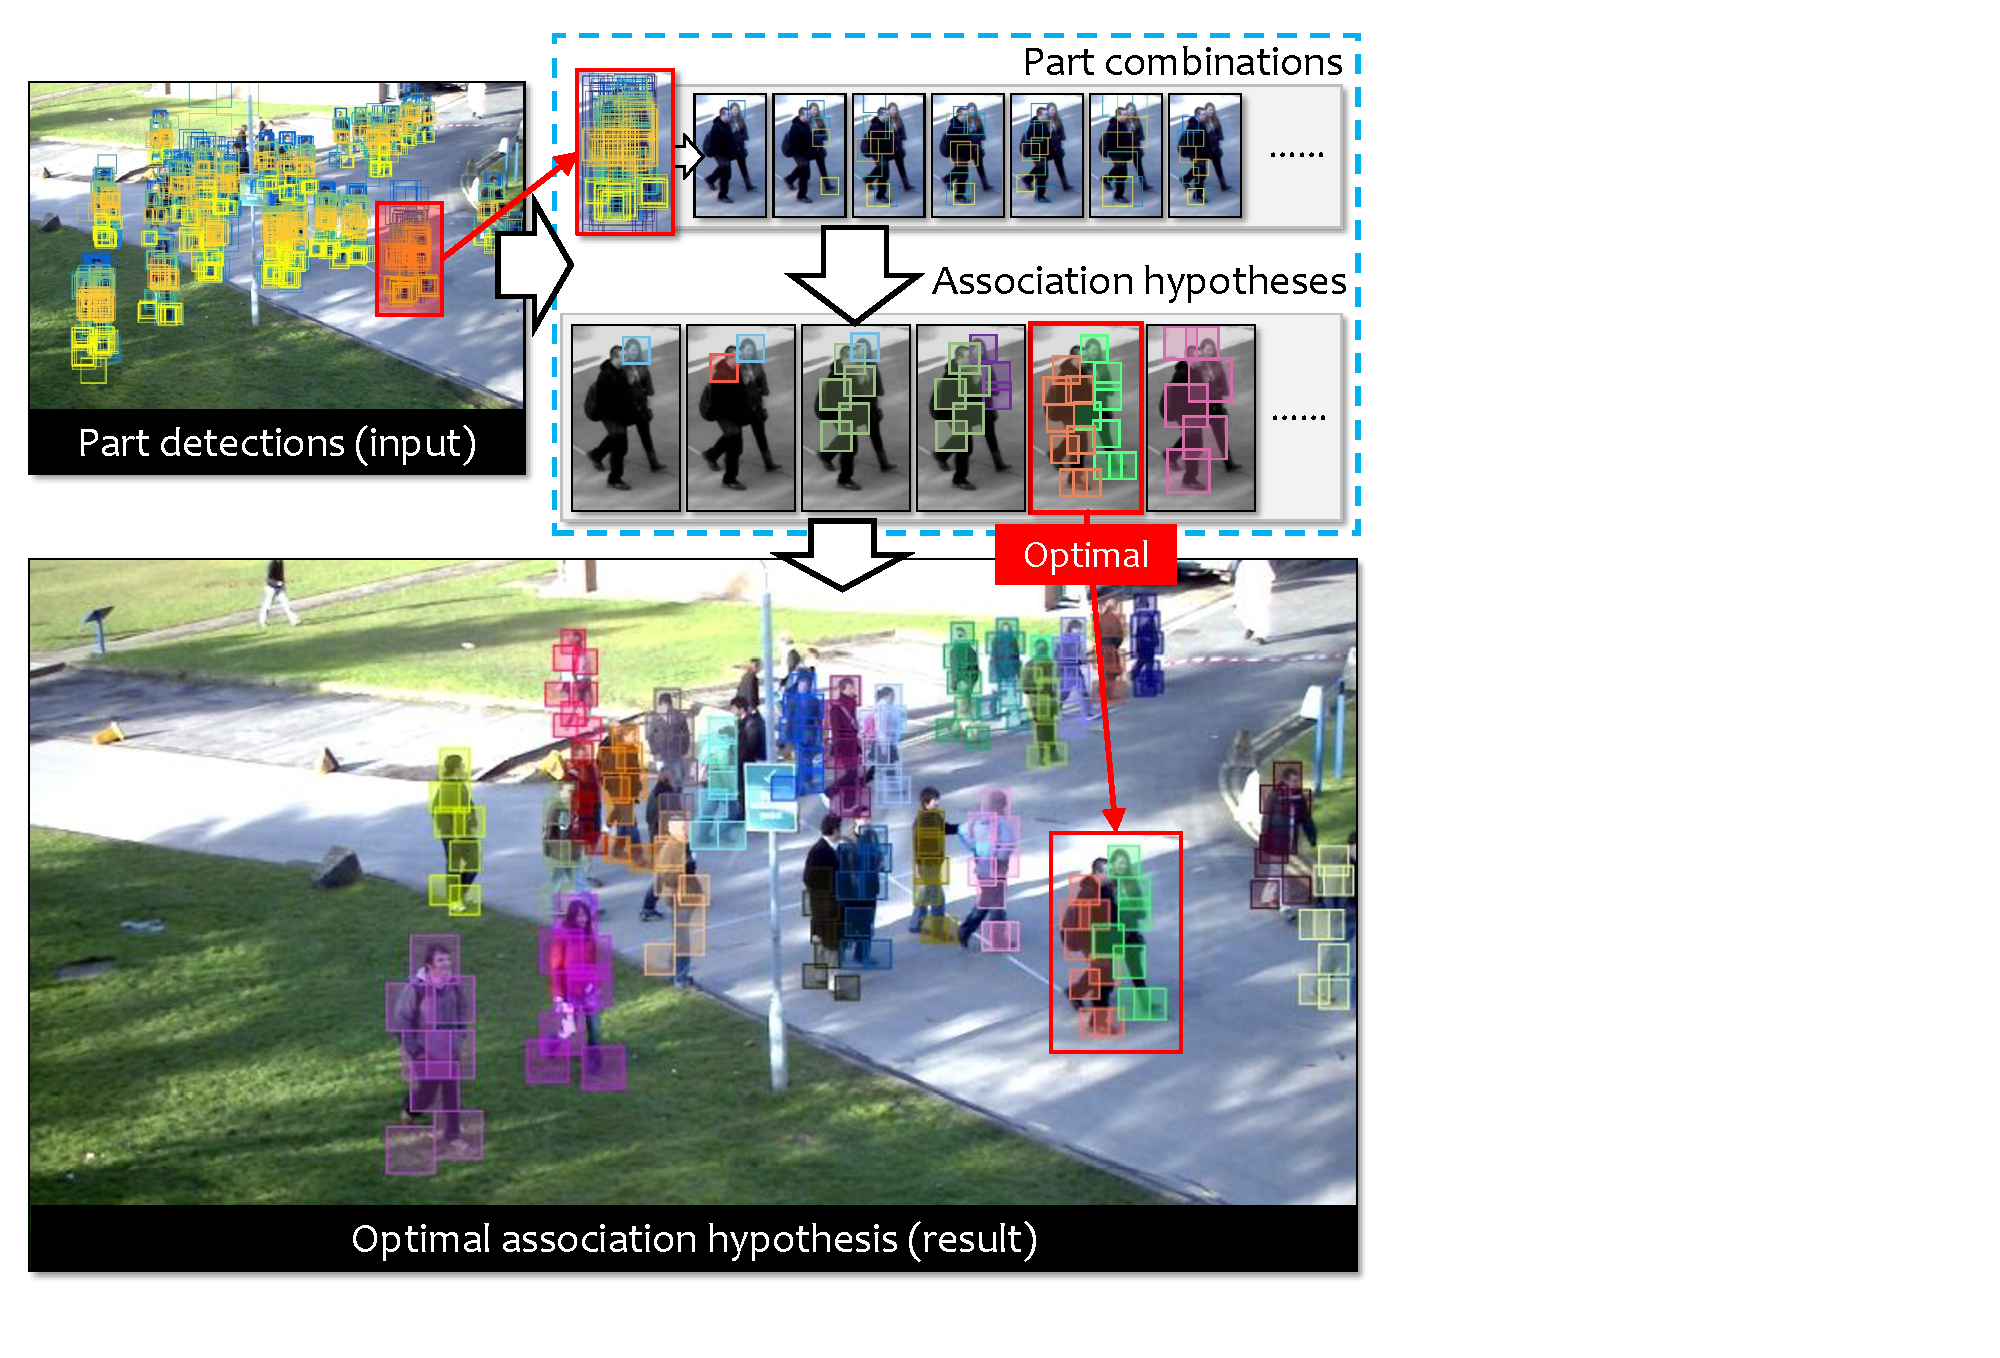
\includegraphics[width=0.98\textwidth]{../figures/teasure.pdf}
   \caption{The overall scheme of the proposed method.}
   \label{fig:overall_scheme}
\end{figure*}

% 왜 이 문제가 중요한가?
The pedestrain detection is essential for many practical applciations like the self-driving car, the visual analytics, robotics, the visual survaillance and etc.
Futhermore, the performance of those applications are deeply affected by the quality of pedestrian detections.
Thus, the pedestrian detection have been studied widely for the last decade.
% (필요성을 조금 더 자세하게 보충 필요)

% 이 문제가 풀리지 않았는가?
% 문제 1) occlusion
Many of recently proposed methods achieved a good performance on the moderate scene~\cite{dalal2005histograms, felzenszwalb2010object, dollar2009integral, DollarECCV2012crosstalkCascades}.
But they have failed on crowd scenes because they only modeled an isolated pedestrian.
They cannot handle the significant variation at the appearance of pedestrians which are occluded by other pedestrians.
% 문제 2) redundancy 제거하는 과정에서 실제 human도 제거되는 문제.
Moreover, they have lost true positive detections during the post processing like non-maximum suppression (NMS), which removes redundant detecions from initial detection result.

% 기존 연구들
In recent years, methods modeling the partially occluded pedestrian, are proposed~\cite{ouyang2013modeling, ouyang2013joint}.
They learned several models representing various partial occlusions of a pedestrian, and detected each models on a target image.
This kind of method can detects more pedestrian candidates than the previous methods.
However, this kind of methods are nothing but the relaxation of joint conditions between body parts.
Thus, they need a training to learn an approperiate threshold value for each occluded pedestrian model, to reduce the number of false positive detections.
This means that the methods always need a training step when they are applied to a new scene, and it narrows the utility of the methods.

% Multi-person case의 detector 학습, 
The alternative methods modeled the mutual occlusions between pedestrians~\cite{ouyang2013single, tang2013learning}.
They modeled typical cases of mutual occlusion scenarios between pedestrians with multiple classifiers.
They achieved a good performance on several scenes which contain the occlusion patterns that are learned by classifiers.
However, it is impossible to model the all of occlusion cases with a fixed number of case studies.
Furthermore, they cannot handle complex occlusions that are related with more than three pedestrians.
This kind of occlusions are usual in severly crowded scenes.
% Global occlusion reasoning 
% (global view, PAMI 2015 논문)

% global optimize
Yan $et al.$~\cite{yan2012multi} proposed the method based on the optimization for high density crowd scene.
In~\cite{yan2012multi}, the spatial relationships between bounding boxes of mutually occluded pedestrians are modeled, and the modeling information was used in the calculation of an optimization cost.
Whenever the test scene has a same scene structure and a resemble density of pedestrians with training scene, the method acquires high recall with high precision in detection.
However, these conditions are unrealistic in general situations because the training at every applying scenes needs too much labor, and the density of pedestrians always varies.

% 내 아이디어를 간단히 설명한다면?
In this paper, we propose the novel pedestrian detection method which considers the overall occlusions in the target image at once.
In our method, we explicitely infer occlusions of each body part, to distinguish detections of partially occluded pedestrians from false positive detections.
Moreover, we provide the confidential appearance of each pedestrian.
For the reasoning of body part occlusions, we formulate the pedestrian detection problem as the part assignment problem, and solve the problem with the binary constrainted quadratic programming (BQP).
When the proposed BQP are solved, the problem of removing redundancy in initial detection results is also resolved.
% The proposed BQP not only infers the occlusion, but also resolves the problem of redundant detections.
In addition, the prior information about occluding area in the target image can be easily unified to our BQP when it is available.
% 실험 결과 요약
Experiments on the public benchmarks show that the proposed method has the robust detection performance and capability to provide the exact appearances of each pedestrian.
% 제시한 방법은 pedestrian detection and tracking에 widely 사용되는 public benchmarks에서 기존의 state-of-the-art 방법들에 비해 강인한 성능을 보여주었다.
%==============================================================================


%%%%%%%%%%%%%%%%%%%%%%%%%%%%%%%%%%%%%%%%%%%%%%%%%%%%%%%%%%%%%%%%%%%%%%%%%%%%%%%
% FORMULATION
%%%%%%%%%%%%%%%%%%%%%%%%%%%%%%%%%%%%%%%%%%%%%%%%%%%%%%%%%%%%%%%%%%%%%%%%%%%%%%%
\section{Formulation}
\label{sec:formulation}
% 입력 -> 출력 간략히 소개
The goal of the proposed method is to generate sets of visible (body) part for each pedestrian on an input image, by assigning an initial (or input) part detections $\mathbf{P}=\{p_1,...,p_K\}$ to each pedestrian.
Each part $p_i = (b_i, t_i, r_i)$ is defined by a bounding box $b_i \in \mathbb{R}^{1\times4}$, a type index $t_i \in \mathbb{N}$, and part filter respose $r_i \in \mathbb{R}$. 
For convenience, we refer to a body part detection as a part in this paper.
In this section, we show how we formulate the part assignment problem as the BQP, and also present the concrete formulation of our BQP.

%==========================================================
% ASSIGNMENT HYPOTHESIS
%==========================================================
\subsection{Part assignment hypothesis}
\label{subsec:part_assignment_hypothesis}
If a pedestrian is fully visible, all of the parts of these pedestrian would be detected.
A structure of those parts can be defined by $\mathbb{N}$-dimensional tuple of part indices, $\omega_i=(i_1,...,i_{\mathbb{N}}), i=1,...,N_{\omega}$, where $N_{\omega}$ is the number of entire possible part assignments.
We call it a part assignment.
Each of element in a part assignment represents the pedestrian's part in a specific type.
To represent a partially occluded pedestrian, an element of a part assignment can be zero, which means there is no proper part in that type for the pedestrian.




We define a part assignment $\omega_i=(i_1,...,i_{n_i}), i=1,...,N_{\omega}$ as a $\mathbb{N}$-dimensional tuple of part indices.
Here, $N_{\omega}$ is the number of entire possible part assignments.


the set of parts which are supposed to be detected from the same pedestrian. $N_{\omega}$ is the number of entire possible part combinations. Becuase a pedestrian has only one in each part type, a part combination is the the subset of input part set $\mathbf{P}$ which contains at most one in each part type.
% the subset of input part set $\mathbf{P}$ a part combination $\omega_i=\{p_{i_1},...,p_{i_{n_i}}\}, i=1,...,N_{\omega}$ and it represents the association between parts.
% 우리는 $\mathbf{P}$의 subset들 중, 동일한 보행자로부터 탐지된 것으로 추정되는 part들로 이루어진 set $\omega_i=\{p_{i_1},...,p_{i_{n_i}}\}, i=1,...,N_{\omega}$를 part combination set(part combination)이라 정의한다.
We also define a (part) association hypothesis $\Omega_k=\{\omega_{k_1},...,\omega_{k_{q_k}}\}, k=1,2,...,N_{\Omega}$ as the set of part combinations and we define the universal set of association hypotheses to $\mathbf{\Omega}$. $N_{\Omega}$ is the cardinality of $\mathbf{\Omega}$.
% 그리고 set of part combinations  $\Omega_k=\{\omega_{k_1},...,\omega_{k_{q_k}}\}, k=1,2,...,N_{\Omega}$를 part association hypothesis(이하 association hypothesis)라 정의하고 이들의 전체 집합을 $\mathbf{\Omega}$라 정의한다.
Then, the data association problem arised between parts is equivalent to the problem of finding the association hypothesis which best describes the target image.
But is also has to be feasible.
To became a feasible association hypothesis, all the part combinations in the association hypothesis must be compatible each other.
We define the compatibility conditions between part combinations in the next paragraph.
% 이 때, association hypothesis가 실제 상황에 맞게끔 feasible하려면 같은 association hypothesis에 속한 part combination들이 서로 coexistence할 수 있어야 한다. 우리는 compatible한 part combinations를 다음 paragraph와 같이 정의한다.

\paragraph{Compatibility of part combinations:} 
In normal situations, people cannot share body parts.
Thus, compatible part combinations $\omega_i$ and $\omega_j$ do not have common parts. 
That is $\omega_i \cap \omega_j = \phi$.
% 하나의 신체 부위를 둘 이상의 pedestrian이 공유할 수 없으므로, 서로 compatible한 part combination들은 common part를 갖고 있지 않아야 한다.
% 즉, 임의의 두 part combination $\omega_i$와 $\omega_j$가 compatible하기 위해서는 $\omega_i \cap \omega_j = \phi$여야 한다.
Moreover, any different parts cannot be seen at a common location in the target image since typical body parts are not transparence.
Thus, we assume that a part combination $\omega_i$ is incompatible to a part combination $\omega_j$ if $\omega_i$ overlaps any part of $\omega_j$.
Let's define the decision function $\delta_c (p_k, \omega_i)$ which examines whether a part $p_k \notin  \omega_i$ is covered by $\omega_i$ as below
% 또한 사람의 신체부위는 투명하지 않으므로 이미지의 한 영역에서 두 사람의 part가 동시에 보일 수 없다.
% $\omega_i$에 포함되지 않는 part $p_k$가 $\omega_i$에 의해 coverd되는지 여부를 판단하는 decision function $\delta_c (p_k, \omega_i)$를 아래와 같이 정의하자
\begin{equation}
   \label{eq:part_occluion}
   % \delta_c (p_k, \omega_i) = \delta \left( \sum_{p_l \in \omega_m} S(b_k \cap b_l) - \theta_{p} \times S(b_k) \right)
   \delta_c (p_k, \omega_i) = \begin{cases}
      1, &\frac{1}{S(b_k)} \sum_{p_m \in \omega_i} S(b_k \cap b_m) \geq \theta_{c},\\
      0, &\mathrm{otherwise},
   \end{cases}
\end{equation}
where $S(b)$ indicates the area of the bounding box $b$ and $b_l \cap b_m$ represents the intersection of $b_l$ and $b_m$. $\theta_{c}$ is the design parameter for the part covering. 
Then, part combinations $\omega_i$ and $\omega_j$ must satisfy the condition in below to be compatible each other
\begin{equation}
   \label{eq:compatible_overlap}
   \sum_{p_m \in \omega_i} \delta_c(p_m,\omega_j) + \sum_{p_k \in \omega_j} \delta_c(p_k,\omega_i) = 0.
\end{equation}
When we define $\mathbb{C}$ as the set of unordered index pairs of compatible part combinations, an association hypothesis $\Omega_l \in \mathbf{\Omega}$ is feasible when it satisfies
\begin{equation}
   \label{eq:feasible_association_hypothesis}
   \{i,j\} \in \mathbb{C}, \forall \omega_i,\omega_j \in \Omega_l.
\end{equation}


%==========================================================
% OPTIMAL HYPOTHESIS
%==========================================================
\subsection{Optimal hypothesis}
\label{subsec:optimal_hypothesis}
In this section, we propose BQP finds the best association hypothesis for the target image.
In our BQP, the score of each association hypothesis is defined by the part combinations in the hypothesis, and the optimal hypothesis is the hypothesis which has the best score.
% 본 section에서는 어떤 association hypothesis가 target image를 잘 설명하는지를 판단하는 근거로써 hypothesis에 속한 part combination들로 정의되는 hypothesis의 score를 제안한다.
% We call the assocation hypothesis that has the best score, the optimal hypothesis.
The score of the hypothesis consists of two score types: the detection score and the occlusion score.
A detection score $\gamma_i$ of the part combination $\omega_i$ depends on the quality of $\omega_i$ and an occlusion score $q_{ij}$ represents the occlusion between $\omega_i$ and $\omega_j$.
% 제안하는 score는 hypothesis에 속한 part combination 자체가 얼마나 좋은지에 대한 detection score of part combination과 part combination들이 mutual occlusion 측면에서 얼마나 reasonable한지를 나타내는 occlusion score between the pair of part combination으로 정의된다.
The concrete definition of each score will be presented in Section~\ref{subsec:score}.
When we define $\mathbf{I}_{\Omega_i}$ as the index set of part combination in $\Omega_i$, the score of the association hypothesis $\Omega_k$ is defined by
% 임의의 part combination $\omega_i$의 detection score를 $\gamma_i$라 하고, 임의의 두 part combinations $\omega_i$ and $\omega_j$간의 occlusion score를 $q_{ij}$라 하면 임의의 association hypothesis $\Omega_k$의 score $\eta_k$는 다음과 같다
\begin{equation}
   \label{eq:hypothesis_score}
   \eta_k = \sum_{i \in \mathbf{I}_{\Omega_k}} \gamma_i + \sum_{i \in \mathbf{I}_{\Omega_k}}\sum_{j \in \mathbf{I}_{\Omega_k}} q_{ij}.
\end{equation}
% Here, $q_{ii}$ represents the score about part missing in $\omega_i$. 각 score의 concrete definition은 Section~\ref{subsec:score}에서 다룬다. (\ref{eq:hypothesis_score})을 이용하여 정의한 아래의 최적화 문제를 풀면, 결과적으로 target image에서의 pedestrian detection 문제를 푸는 것이 된다.
Then, solving the part association problem can be described by the optimizaion problem finding the hypothesis with the best score as below
\begin{equation}
   \label{eq:pedestrian_optimization}
   \begin{aligned}
      \Omega^* = \argmax_{\Omega_k \in \mathbf{\Omega}} & \sum_{i \in \mathbf{I}_{\Omega_k}} \gamma_i + \sum_{i \in \mathbf{I}_{\Omega_k}} \sum_{j \in \mathbf{I}_{\Omega_k}} q_{ij}\\
                 s.t. & \; \{i, j\} \in \mathbb{C}, \; \forall i,j \in \mathbf{I}_{\Omega_k}.
   \end{aligned}
\end{equation}

We reformulate Eq.~(\ref{eq:pedestrian_optimization}) to the BQP because there are plenty of effective solving algorithms have been proposed for a BQP.
% 우리는 이를 mathematically equivalent하고 기존에 많은 solver가 제시된 formulation인 binary quadratic programming (BQP)으로 re-formulate하였다. 
Let's define $Q \in \mathbb{R}^{N_{\omega} \times N_{\omega}}$ as below
\begin{equation}
   \label{eq:Q}
   [Q]_{ij} = 
      \begin{cases}
         q_{ij},            & i \neq j, \\
         q_{ii} + \gamma_i, & otherwise.
      \end{cases}
\end{equation}
Then, the BQP in below is mathematically equivalent to Eq.~(\ref{eq:pedestrian_optimization}).
\begin{equation}
   \label{eq:quadratic_programming}
   \begin{aligned}
      \mathbf{x}^* = \argmax_{\mathbf{x}} & \quad \mathbf{x}^T Q \mathbf{x} \\
                                     s.t. & \quad x_i + x_j \leq 1, \; \forall \{i,j\} \notin \mathbb{C} \\
                                          & \quad x_i \in \{0,1\},
   \end{aligned}
\end{equation}
where $\mathbf{x} \in \{0,1\}^{N_{\omega} \times 1}$ indicates the vector of decision variables $x_i$ which represents the selection of $w_i$ in the optimal association hypothesis.
% $\bar{\mathbb{C}} = \{\{i,j\}|\forall\{i,j\}\notin\mathbb{C} \; \mathrm{for} \; i,j=1,...,N_{\omega}\}$는 incompatibility set이다. 
% 우리는 Branch and bound(이름과 참고문헌확인요망)를 기반으로 (\ref{eq:quadratic_programming})를 exact하게 푼다. 
% 이를 통해 구해지는 optimal hypothesis는 다음과 같다.
That is, the optimal hypothesis is defined by
% 즉, (\ref{eq:quadratic_programming})을 풀어 얻은 optimal hypothesis는 다음과 같이 표현할 수 있다.
\begin{equation}
   \label{eq:optimal_hypothesis}
   \Omega^* = \{\omega_i | x_i^* = 1\}.
\end{equation}

%==========================================================
% DECOMPOSITION
%==========================================================
\subsubsection{Problem decomposition}
\label{subsubsec:problem_decomposition}
The exact solving of Eq.~(\ref{eq:quadratic_programming}) requires the huge number of computations when the number of part combinations increases because the computational complexity of Eq.~(\ref{eq:quadratic_programming}) is exponential to the number of optimization variables.
% (\ref{eq:quadratic_programming})과 같은 BQP을 exact하게 푸는 것은 매우 큰 계산량을 요구한다.
% 특히, BQP의 계산량은 optimization variable의 개수, 즉 part combination의 개수에 따라 지수적으로 증가하기 때문에 큰 수의 part combination은 매우 큰 계산량을 요구한다.
However, it is unavoidable to generate a number of part combinations in crowd scenes.
% To resolve this problem, we construct sub-problems of Eq.~(\ref{eq:quadratic_programming}) by partitioning  optimization variables in Eq.~(\ref{eq:quadratic_programming}) according to their relationship.
% That means that optimization variables from different sub-problems do not effect each other in Eq.~(\ref{eq:quadratic_programming}).
To resolve this problem, we construct sub-problems of Eq.~(\ref{eq:quadratic_programming}) whose optimization variables are indepedent to those of other sub-problems.
After solving those sub-problems, we merge their solutions to generate the solution of Eq.~(\ref{eq:quadratic_programming}).
% by partitioning the entire part combinations into subsets whose part combinations are independent to those of other subsets.
% we partition the entire part combinations into sets of part combinations coupled  in the optimization.
% Then, we construct sub-problems for each set as defined in Eq.~(\ref{eq:quadratic_programming}) and merge their solutions to generate the final solution.
% 우리는 이러한 계산량 문제를 moderate하기 위해 전체 part combination에서 서로 독립적으로 풀 수 있는 group들을 찾고 각 group별로 (\ref{eq:quadratic_programming})의 sub-problem을 생성 및 풀이하는 방법을 제안한다.
In typical cases, the size of each set is relatively smaller than the number of entire part combinations, $N_{\omega}$.
Therefore, even we have to solve BQP multiple times, solving sub-problems needs much less computations then the original BQP.
% sub-problem에서 고려하는 part combination의 수는 전체 part combination의 수보다 상대적으로 작기 때문에 복수의 sub-problem을 푼다고 하여도 전체 계산량 측면에서 유리하다.

% 우리는 다음의 방법으로 (\ref{eq:quadratic_programming})에서 서로 연관을 갖는 optimization variable의 group을 찾는다.
In Eq.~(\ref{eq:quadratic_programming}), optimization variables depend each other are the variables corresponds to part combinations which are incompatible or in an occlusion relationship.
% 서로 연관을 갖는 optimization variable들은 서로 occlude 가능하거나 혹은 서로 공존할 수 없는 part combination들에 대응되는 variable들이다.
% 이는 $Q$ matrix에서 non-zero off-diagonal score를 갖는 variable pair나 서로 incompatible한 part combination에 대응되는 variable pair들이다.
To reveal these relationship between optimization variables, we define a new score matrix $Q_{\bar{\mathbb{C}}} \in \mathbb{R}^{N_{\omega} \times N_{\omega}}$ as
% 우리는 이러한 연관성을 하나의 matrix로 표현하기 위해 아래와 같이 $Q_{\bar{\mathbb{C}}}$를 다음과 같이 정의한다.
\begin{equation}
   \label{eq:Q_incompatible}
   [Q_{\bar{\mathbb{C}}}]_{ij} = 
   \begin{cases}
      -1        & \{i,j\} \notin \mathbb{C}, \\
      [Q]_{ij}, & \mathrm{otherwise}.
   \end{cases}
\end{equation}
Then, with the block diagonalization, get the permutation matrix $P_b \in \mathbb{R}^{N_{\omega} \times N_{\omega}}$ and the block diagonal matrix $Q_b \in \mathbb{R}^{N_{\omega} \times N_{\omega}}$ which satisfy the equation below
% 이 후, 이를 block diagonalization을 통하여 permutation matrix $P_b$와 block diagonal matrix $Q_b$를 구한다.achieve
\begin{equation}
   \label{eq:Q_bd}
   Q_b = P_b \times Q_{\bar{\mathbb{C}}} = \mathrm{diag}(Q_{b,1},...,Q_{b,m}).
\end{equation}
Then, the sets of optimization variables correspond to each $Q_{b,i}$ can be solved independently.
When we define the solution of each $Q_{b,i}$ to $\mathbf{x}_{b,i}^*$, the solution of the original BQP, Eq.~(\ref{eq:quadratic_programming}) can be achieved by
% 이를 이용하여 part combination들을 $m$개의 group으로 나눈 후, 각각에 대해 BQP를 생성하여 solution $\mathbf{x}_{b,i}^*$을 얻으면 아래와 같은 방법으로 (\ref{eq:quadratic_programming})를 직접 풀어서 얻는 solution $\mathbf{x}^*$을 얻을 수 있다.
\begin{equation}
   \label{eq:solution_merge}
   \mathbf{x}^* = P_b^T (\mathbf{x}_{b,1}^{*T}, ..., \mathbf{x}_{b,m}^{*T})^T.
\end{equation}
%==============================================================================



%%%%%%%%%%%%%%%%%%%%%%%%%%%%%%%%%%%%%%%%%%%%%%%%%%%%%%%%%%%%%%%%%%%%%%%%%%%%%%%
% PART COMBINATION
%%%%%%%%%%%%%%%%%%%%%%%%%%%%%%%%%%%%%%%%%%%%%%%%%%%%%%%%%%%%%%%%%%%%%%%%%%%%%%%
\section{Part combination}
\label{sec:part_combination}
In this section, we describe the generation of part combinations and shows the concrete definition of two types of score: the detection score and the occlusion score. We also explain how to unify the occlusion prior into our optimization when the prior is available.
% 본 장에서는 입력 $\mathbf{P}$로부터 part combination들을 어떻게 생성하는지와, 이들에 의해 정의되는 detection, occlusion score에 대해 concrete하게 정의한다. 또한, occlusion prior가 available할 시 이를 어떻게 occlusion score에 반영하는지도 설명한다.

%==========================================================
% GENERATION
%==========================================================
\subsection{Generation}
\label{subsec:generation}
% feasible한 part association에 대하여
As mentioned in Section~\ref{subsec:part_assocation_hypothesis}, a part combination is the set of parts which are supposed to be from same pedestrian.
% 에서 언급한 바와 같이 part combination은 하나의 보행자로부터 탐지된 것으로 추정되는 part들의 집합이므로 우리는 part combination 내 part들은 다음 세 가지 조건을 만족할 것이라 가정하였다.
Thus, we assume that part combinations must satisfy three conditions.
First, all part combinations must have a head part because heads are less occluded than other part types in tipycal cases.
Second, a part combination have at most one part in each part type because a human cannot have duplicated parts.
Last, locations of missed parts in a part combination can be estimated by the deformation model with already parts included in the part combination because a human cannot deforms severely.
% 첫 째, 한 사람이 한 종류의 신체부위를 두 개 이상 가질 수 없으므로, 동일한 type의 part 두 개 이상이 하나의 part combination으로 묶이지 않을 것이다.
% 둘 째, pedestrian의 deformation이 급격하지 않을 것이라 가정하고, type에 따른 part의 위치가 어느정도 일정한 범위 내에서만 변동될 것이다.
% 마지막으로, 우리는 pedestrian이 탐지될 때, head는 반드시 보일 것이라 가정하고, 모든 part combination에 head가 포함도록 하였다.
% 입력 part에 대한 더 자세한 설명
Based on theses conditions, we generate part combinations from $\mathbf{P}$ in the following way.

% part clustering by its type
At first, we seperate $\mathbf{P}$ into $\mathbf{P}_t, t=1,...,N_p$ according to their types.
$N_p$ represents the number of available part types in $\mathbf{P}$.
Since a head is more rigid than other parts, we apply Non-Maximum Suppression (NMS) to the head set with the maximum overlap ratio $\theta_{h}$ for reducing the number of incompatible part combinations.
% 먼저 $\mathbf{P}$에서 head들만을 추린 후, the maximum overlap ratio $\theta_{h}$로 non-maximal supression(주석정리요망)을 적용하여 candidate head set $\mathbf{P}_1$을 생성한다.
% 그리고 $\mathbf{P}$ 중 head를 제외한 나머지 part들을 type에 따라 $\mathbf{P}_t, t=2,...,N_p-1$로 partitioning한다.
After NMS, we generate part combinations by adding or omitting the associable parts from each $\mathbf{P}_t$.
Since all part combinations must include a head part, the number of possible cases of part type inclusion is $2^{N_p-1}$.
To determine an associability between the parts in an arbitrary part combination $\omega_i$, we borrowed the star-model from the Deformable Part Model (DPM)~\cite{felzenszwalb2010object}.
By voting with parts in $\omega_i$, we estimate the fullbody of pedestrian for $\omega_i$, $\tilde{p}_{i_0} = (\tilde{b}_{i_0},0,0)$ which is known as a root part in \cite{felzenszwalb2010object}.
Then we get $\tilde{p}_{i_t} = (\tilde{b}_{i_t},t,0)$, the desired location of part type $t$ from the perspective of $\tilde{p}_{i_0}$.
With $\tilde{p}_{i_t}$ we determine the part $p_{i_t}$ is associable with other parts in $\omega_i$ when it satisfies the condition below
\begin{equation}
   \label{eq:association}
   \frac{\norm{l_c(b_{i_t}) - l_c(\tilde{b}_{i_t})}_2}{\sqrt{S(b_{i_t}) \cdot S(\tilde{b}_{i_t})}}  \leq \theta_d, \forall p_{i_t} \in \omega_i.
\end{equation}
where $l_c(b_j) = (u_j,v_j)$ represents the image coordinates of the center point of the box $b_j$ and $\theta_d$ is the design parameter.
We regard $\omega_i$ as a valid part combination when all of its parts satisfy Eg.~\ref{eq:association}.
After generating the part combinations, we only left the valid part combinations for the optimzation.
% 다음으로, 각 head들 $p_{i_1} \in \mathbf{P}_1$에 대해 deformation condition을 기반으로 각 $\mathbf{P}_t$에서 associate 가능한 part들을 추려내어 fullbody에 대한 part combination들 $\omega_{f_j},j=1,...,N_f$을 생성한다.
% the deformation condition은 DPM(주석)에서 차용하였다.
% 이 후, 각 $\omega_{f_j}$의 subset 중 head를 포함하는 subset들을 partially occluded된 pedestrian에 대한 part combination들로 삼는다.
% 우리는 임의의 part combination $\omega_m$에 어떠한 type의 part가 포함되는지에 대한 정보를 configuration이라 부르고 이를 다음과 같이 정의되는 binary vector $\mathbf{c}_m \in \{0,1\}^{N_p \times 1}$으로 표현한다.
% \begin{equation}
%    \label{eq:configuration}
%    c_{m,t} = \begin{cases}
%       1, & \mathbf{P}_t \cap \omega_m \neq \phi, \\
%       0, & \mathrm{otherwise}.
%    \end{cases}
% \end{equation}
% 이 때, fullbody part combination $\omega_{f_j}$로부터 파생되는 part combination들은 다음의 두 조건에 따라 생성하였다.
% 첫 째로, $\omega_{f_j}$내 part 중, $\omega_{f_j}$와 compatible한 다른 part combination들의 part들 중 그 어떠한 것도 해당 part를 가리지 않는다면 해당 part를 포함하는 configuration만 이용하여 part combination들을 생성한다.
% 두 번째로, 첫 번째 조건을 제외하고는 항상 head로부터 Figure~(아직안그림)에 따라 연결 가능한 part들이 포함되는 configuration들만 이용하여 part combination들을 생성한다.
% 이러한 과정을 Figure~\ref{fig:part_association}에 도시하였다.

%==========================================================
% PRUNING
%==========================================================
\subsection{Pruning}
\label{subsec:pruning}
% SVM 적용 이유와 효과
Reducing the number of part combinations is critical for the compuational complexity of our optimization as mentioned in \ref{subsubsec:problem_decomposition}.
Futhermore, the performance of the proposed method can be dameged if the inferior part combinations overwhelm those from real pedestrians with their number.
Thus, the pruning of part combination is required for both the performance and the efficiency.
% 앞 서 \ref{subsubsec:problem_decomposition}에서 언급한 것과 같이 part combination의 수는 계산량에 큰 영항을 미친다.
% 이와 덜불어, 제안하는 방법은 part combination을 기반으로 occlusion 및 localization에 대한 inferencing 하기때문에 
% part combination들에 대해 validation을 수행하는 것이 필요하다.
At the pruning of part combinations, we use the Support Vector Machines (SVM)~\cite{cortes1995support} trained for each case of the part type inclusion.
We represent a case of the part type inclusion as a set of type index $c_k, k=1,...,2^{N_p-1}$ and we call these sets configurations.
To train the SVM of the configuration $c_k$, we generate the samples of part combinations which have $c_k$ as their configuration.
$\mathbf{f}_i$, the sample of an arbitrary part combination $\omega_i$ is defined by
\begin{equation}
   \label{eq:svm_sample_vector}
   \mathbf{f}_i = (r_{i_1}+d_{i_1}(\tilde{b}_{i_1}), ..., r_{i_{|\omega_i|}}+d_{i_{|\omega_i|}}(\tilde{b}_{i_{|\omega_i|}}))^T,
\end{equation}
where $d_{i_t}(\tilde{b}_{i_t})$ is the deformation score of the part $p_{i_t} $ defined in \cite{felzenszwalb2010object}. 
$x_{i_t},y_{i_t}$ and $\mathbf{v}_t$ in \cite{felzenszwalb2010object} are correspond to $u_{i_t},v_{i_t}$ and $l_c(\tilde{b}_{i_t})$ in this paper, respectively.
Since the samples in a higher dimension space are more discriminative than those in a lower dimensional space, we give the higher cost of miss classification about false positives to the SVM of the configuration which has more part types.
That is, the configuration $c_k$ has the cost about false positives $\lambda_k$ as below
\begin{equation}
   \label{eq:svm_fp_cost}
   \lambda_k = \lambda_{1} \cdot \frac{|c_k|}{N_p} + \lambda_{2},
\end{equation}
where $|c_k|$ is the cardinality of $c_k$. $\lambda_{1}$ and $\lambda_{2}$ are design parameters and we used one and zero in our experiments, respectively.

% 일반적인 fullbody detection들은 단일한 thresholding을 통해 유효한 detection과 그렇지 않은 detection을 구분할 수 있지만 제안하는 방법에서 생성하는 part combinations들은 다양한 configuration을 갖고있기 때문에 configuration에 따라 validation 조건을 달리 부여해야 한다.
% 이를 위해 우리는 configuration별로 part filter response와 deformation score를 기반으로 하는 support vector machine (SVM) (주석달것)을 학습하고, 이를 통해 사전 classification을 수행, false positive로 의심되는 part detection들을 제거한다. 
% 우리는 part combination $\omega_i$에 대해 sample vector $\mathbf{f}_i \in \mathbb{R}^{|\omega_i| \times 1}$를 아래와 같이 구성한다.
% \begin{equation}
%    \label{eq:svm_sample_vector}
%    \mathbf{f}_i = (r_{i_1}+d_{i_1}, ..., r_{i_{|\omega_i|}}+d_{i_{|\omega_i|}})^T
% \end{equation}
% 즉, configuration에 포함되는 part의 개수에 따른 차원을 갖는 sample vector들을 생성한다.
% 우리는 part detector를 학습한 dataset에서 각각의 configuration에 대해서 이러한 방식으로 training sample vector들을 생성하여 SVM을 학습한다.
% 이 때, 적은 수의 part를 포함하고 있는 configuration에서도 precision을 유지하기 위해서 configuration에 포함되는 part type의 수가 적을수록 SVM learning 시 false positive에 대한 miss classification cost를 크게 준다. 
% 즉, part의 개수가 $n$개인 configuration에 대해 false positive cost $\zeta_{fp}(n)$를 다음과 같이 부여한다.
% \begin{equation}
%    \label{eq:svm_fp_cost}
%    \zeta_{fp}(n) = \alpha_{fp} \times (1 - \frac{n}{N_p}) + \beta_{fp},
% \end{equation}
% where $\alpha_{fp}$ and $\beta_{fp}$ are design parameters and we used 100 and one in our experiments, respectively.


%==========================================================
% SCORE DESIGN
%==========================================================
\subsection{Score design}
\label{subsec:score}
We evaluate the detection quality of a part combination with the the number and the filter responses of parts in the part combination.
The detection score $\gamma_i$ of an arbitrary part combination $\omega_i$ is defined by
% 우리는 part가 많이 포함될수록, 그리고 각 part의 filter response 및 deformation score가 좋을수록 해당 part combination이 좋은 quality를 갖는다고 정의한다.
% 즉, 임의의 part combination $\omega_i$의 detection score $\gamma_i$는 $\omega_i$의 크기, $\omega_i$에 속한 part들의 filter response 및 deformation score을 기반으로 다음과 같이 정의된다
\begin{equation}
   \label{eq:part_detection_score}
   \gamma_i =\frac{|w_i|^2}{N_p^2}  + \sum_{k \in \mathbf{I}_{\omega_i}} \left( r_k + d_k(\tilde{b}_k) \right),
\end{equation}
where $\mathbf{I}_{\omega_i}$ indicates the index set of parts in $\omega_i$. $d_k(\tilde{b}_k)$ indicates the deformation score of part $p_k$ reference to the root part of $\omega_i$ as described in the previous section.

% occlusion score 설명
The occlusion scores depend on the reason of part missings in the part combination.
We give the penalty to the part combination for a part missing, but the penalty is reduced when the part missing is cause by the occlusion by the other part combination which in the same association hypothesis.
If the type $m$ part is not included in $\omega_i$, the estimated part of type $m$, $\tilde{p}_{i_k} = (\tilde{b}_{i_k},m,0)$ is found by the method mentioned in Section~\ref{subsec:generation} to examine whether the missed part is occluded by other part combinations or not.
Let's define the set of estimated parts of $\omega_i$ as 
\begin{equation}
   \label{eq:estimated_part_set}
   \bar{\omega}_i = \{ \tilde{p}_{i_k} | t_{i_k} \notin c(\omega_i) \},
\end{equation}
where $c(\omega_i)$ indicates the configuration of $\omega_i$.
Then the self occlusion score of $\omega_i$, $q_{ii}$ is defined as below
\begin{equation}
   \label{eq:missing_score}
   q_{ii} = q_i = q(\bar{\omega}_i, \omega_i) = |\omega_i| - N_p = - |\bar{\omega}_i|.
\end{equation}
And the occlusion score of $\omega_i$ by $\omega_j$, $q_{ij}$ is defined by the number of parts in $\bar{\omega}_i$ which are supposed to be occluded by $\omega_j$. 
That is,
\begin{equation}
   \label{eq:covering_score}
   q_{ij} = q(\bar{\omega}_i, \omega_j) = \sum_{\tilde{p}_{i_t} \in \bar{\omega}_i} \delta_c(\tilde{p}_{i_t}, \omega_j).
   % q_{ij} = q(\bar{\omega}_i, \omega_j) = \sum_{k \in \mathbf{I}_{\bar{\omega}_i}} \sum_{m \in \mathbf{I}_{\omega_j}} f(\tilde{b}_{k}, b_{m}, \theta_{o}),
\end{equation}
Here, the function $\delta_c(\tilde{p}_{i_t}, \omega_j)$ is defined in Eq.~\ref{eq:part_occluion}.

% Occlustion score는 part combination들의 part missing이 어떤 요인에 의해 일어났는지에 따라 정의된다.
% 즉, part combination에서 누락되는 type의 part가 있을 시, 이에 대해 penalty를 부여하되, 만약 이러한 part missing이 같은 association hypothesis 내 다른 part combination의 part들로 인한 occlusion 때문이라면 penalty를 줄여주도록 정의한다.
% 우리는 이것을 위해 각 part combination에서 누락된 part의 위치를, deformation을 기반으로 추정하고, 추정된 part가 다른 part combination에 의해 covered되었는지를 판단한다.
% 임의의 part combination $\omega_i$에서 누락된 $t$번째 type의 part에 대한 추정결과를 $\tilde{p}_{i_t} = (\tilde{b}_{i_t},t,0)$라 정의하자.
% $\omega_i$에서 누락된 모든 type의 part들에 대한 추정 모음을 $\bar{\omega}_i = \{ \tilde{p}_{i_t} | c_{i,t} = 0 \}$라 정의하면, $\omega_i$ 자체에 대한 occlusion score $q_{ii}$는 다음과 같이 정의된다
% \begin{equation}
%    \label{eq:missing_score}
%    q_{ii} = q_i = q(\bar{\omega}_i, \omega_i) = |\omega_i| - N_p = - |\bar{\omega}_i|.
% \end{equation}
% Target image에서 $\bar{\omega}_i$ 속 part들의 위치에 $\omega_i$와 compatible한 또다른 part combination $\omega_j$의 part들이 위치할 경우, 이에 의한 occlusion score $q_{ij}, i \neq j$는 다음과 같이 정의된다
% \begin{equation}
%    \label{eq:covering_score}
%    q_{ij} = q(\bar{\omega}_i, \omega_j) = \sum_{\tilde{p}_{i_t} \in \bar{\omega}_i} \delta_c(\tilde{p}_{i_t}, \omega_j).
%    % q_{ij} = q(\bar{\omega}_i, \omega_j) = \sum_{k \in \mathbf{I}_{\bar{\omega}_i}} \sum_{m \in \mathbf{I}_{\omega_j}} f(\tilde{b}_{k}, b_{m}, \theta_{o}),
% \end{equation}

\paragraph{Occlusion prior:}
When the prior information about the occlusions by obstacles or the background is available, we can count the prior information by modifying our self occlusion score in the following way.
% 만약 영상 내 장애물등에 의해 occlusion이 발생할 수 있는 영역 정보를 prior로 취득할 수 있다면, 제안하는 method는 이를 occlusion score에 간단히 통합할 수 있다.
If the binary mask $M_o$ presents the possible occluding areas in the target image, the modified self occlusion score $q_{ii}^+$ of the part combination $\omega_i$ is defined by
% Occlusion prior에 의해 이미지 상 가려짐이 발생할 수 있는 영역에 대한 binary mask $M_o$가 주어졌다면 Eq.~(\ref{eq:missing_score})을 다음과 같이 수정함으로써 이를 occlusion score에 반영할 수 있다.
\begin{equation}
   \label{eq:occlusion_prior_score}
   q_{ii}^+ = q_{ii} + \sum_{\tilde{p}_{i_t} \in \bar{\omega}_i} \delta_{op}(\tilde{p}_{i_t}, M_{op}),
\end{equation}
where $\delta_{op}(\tilde{p}_{i_t}, M_{op})$ is the decision fuction defined by
\begin{equation}
   \label{eq:occlusion_prior_count_function}
   \delta_{op}(\tilde{p}_{i_t}, M_{op}) = 
    \begin{cases}
      1 & \text{if $\frac{|M_{op}(\tilde{b}_{i_t})|}{S(\tilde{b}_{i_t})} > \theta_c $}, \\
      0 & \text{otherwise}.
   \end{cases}
\end{equation}
Here, $|M_{op}(\tilde{b}_{i_t})|$ indicates the number of ones in the region defined by $\tilde{b}_{i_t}$ on $M_{op}$.
%==============================================================================



%%%%%%%%%%%%%%%%%%%%%%%%%%%%%%%%%%%%%%%%%%%%%%%%%%%%%%%%%%%%%%%%%%%%%%%%%%%%%%%
% EXPERIMENTS
%%%%%%%%%%%%%%%%%%%%%%%%%%%%%%%%%%%%%%%%%%%%%%%%%%%%%%%%%%%%%%%%%%%%%%%%%%%%%%%
\section{Experiments}
\begin{figure}[t]
   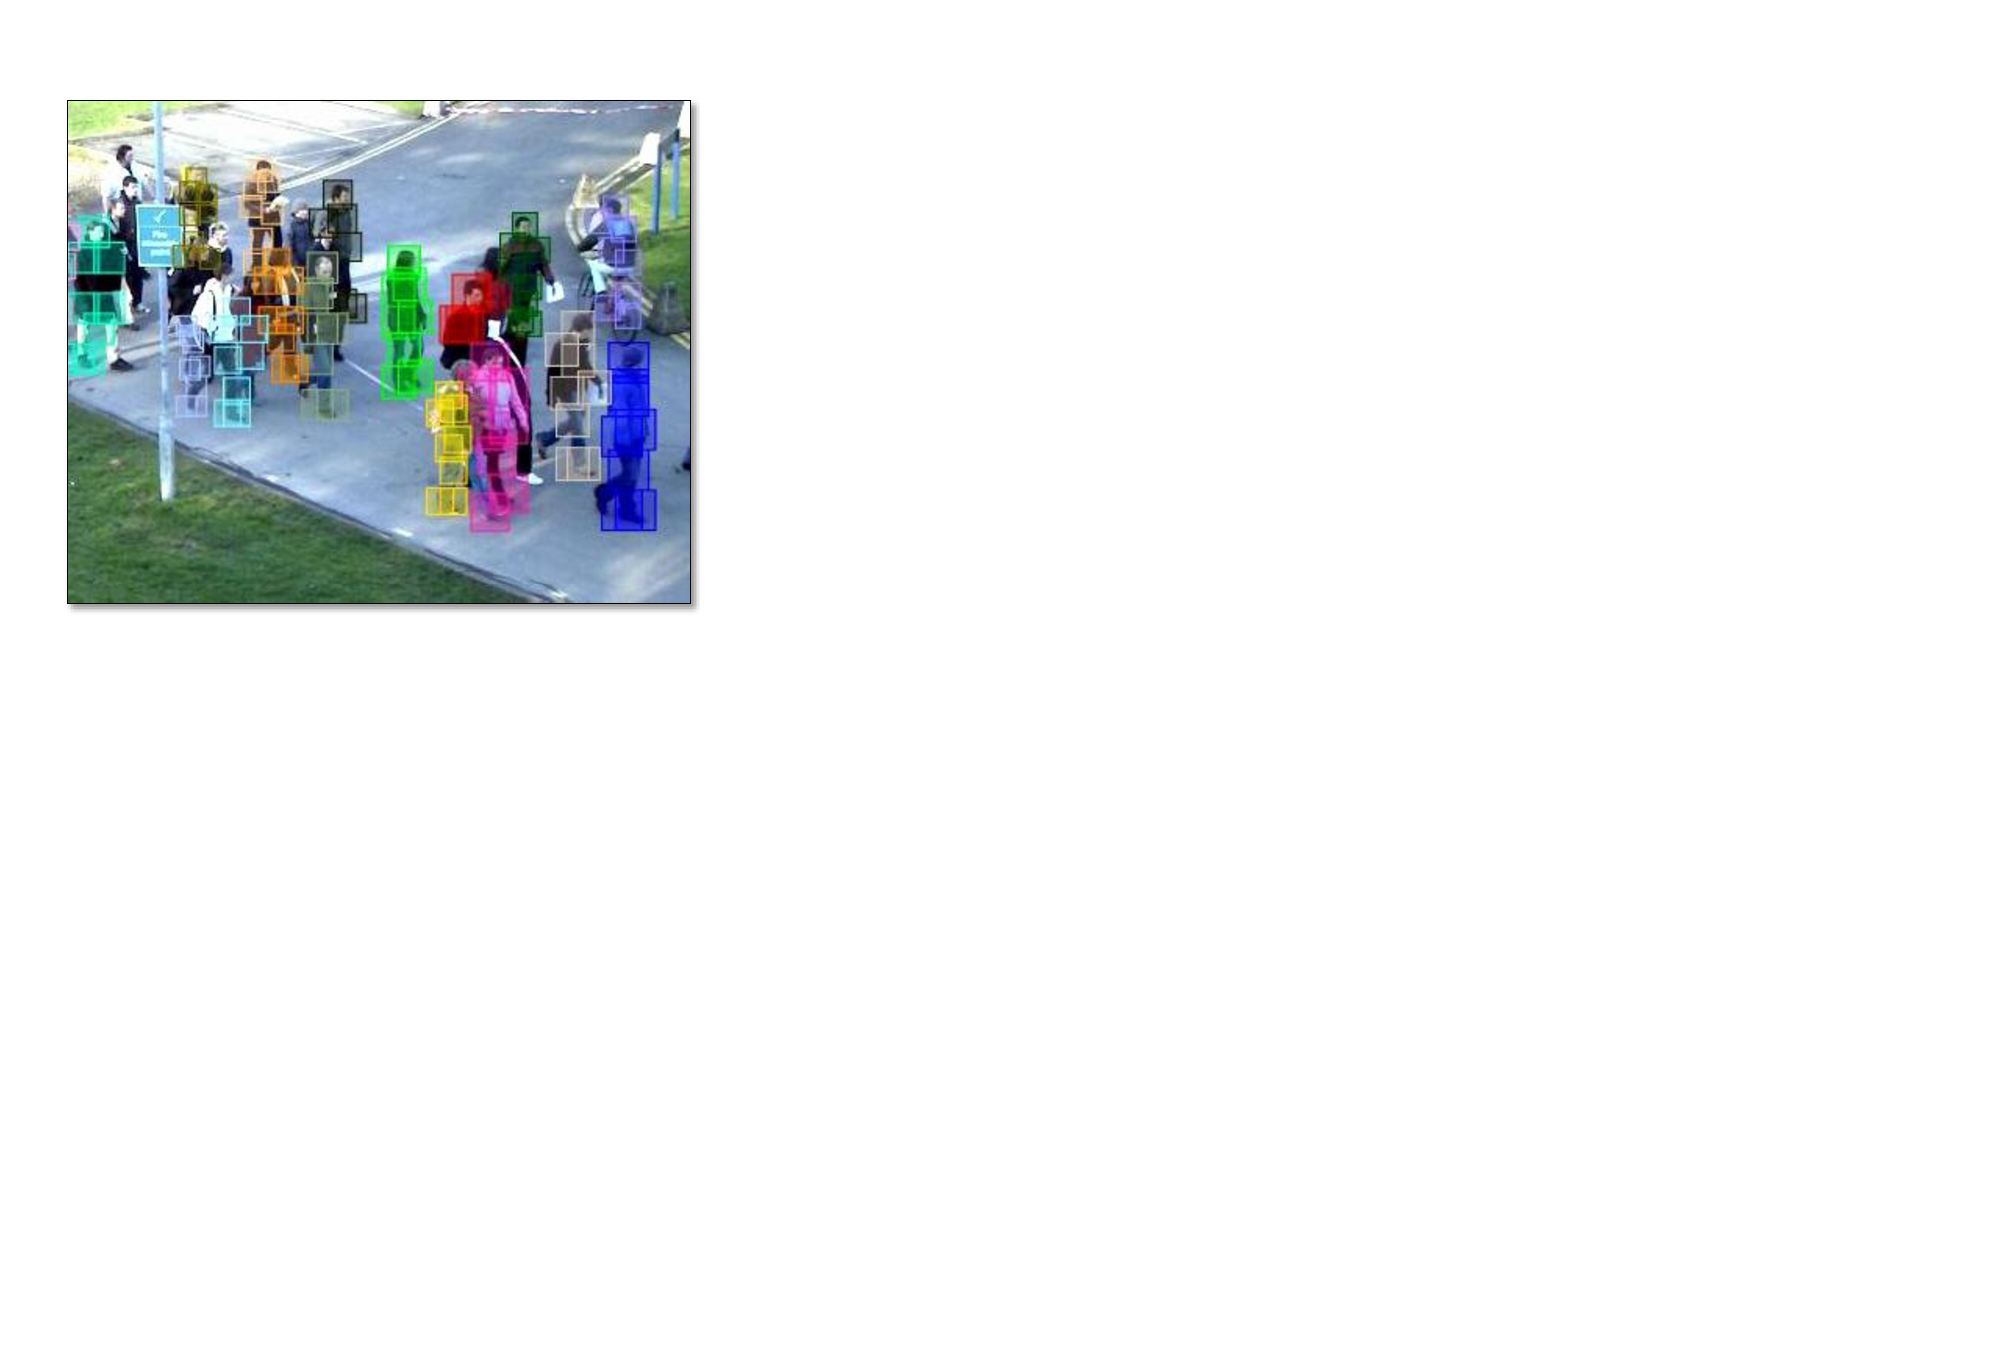
\includegraphics[width=0.48\textwidth]{../figures/visible_part_association.pdf}
   \caption{Sample of visible part association from PEST2009 S2.L3.}
   \label{fig:visible_part_association}
\end{figure}

\label{sec:experiments}
\begin{figure*}[t]
   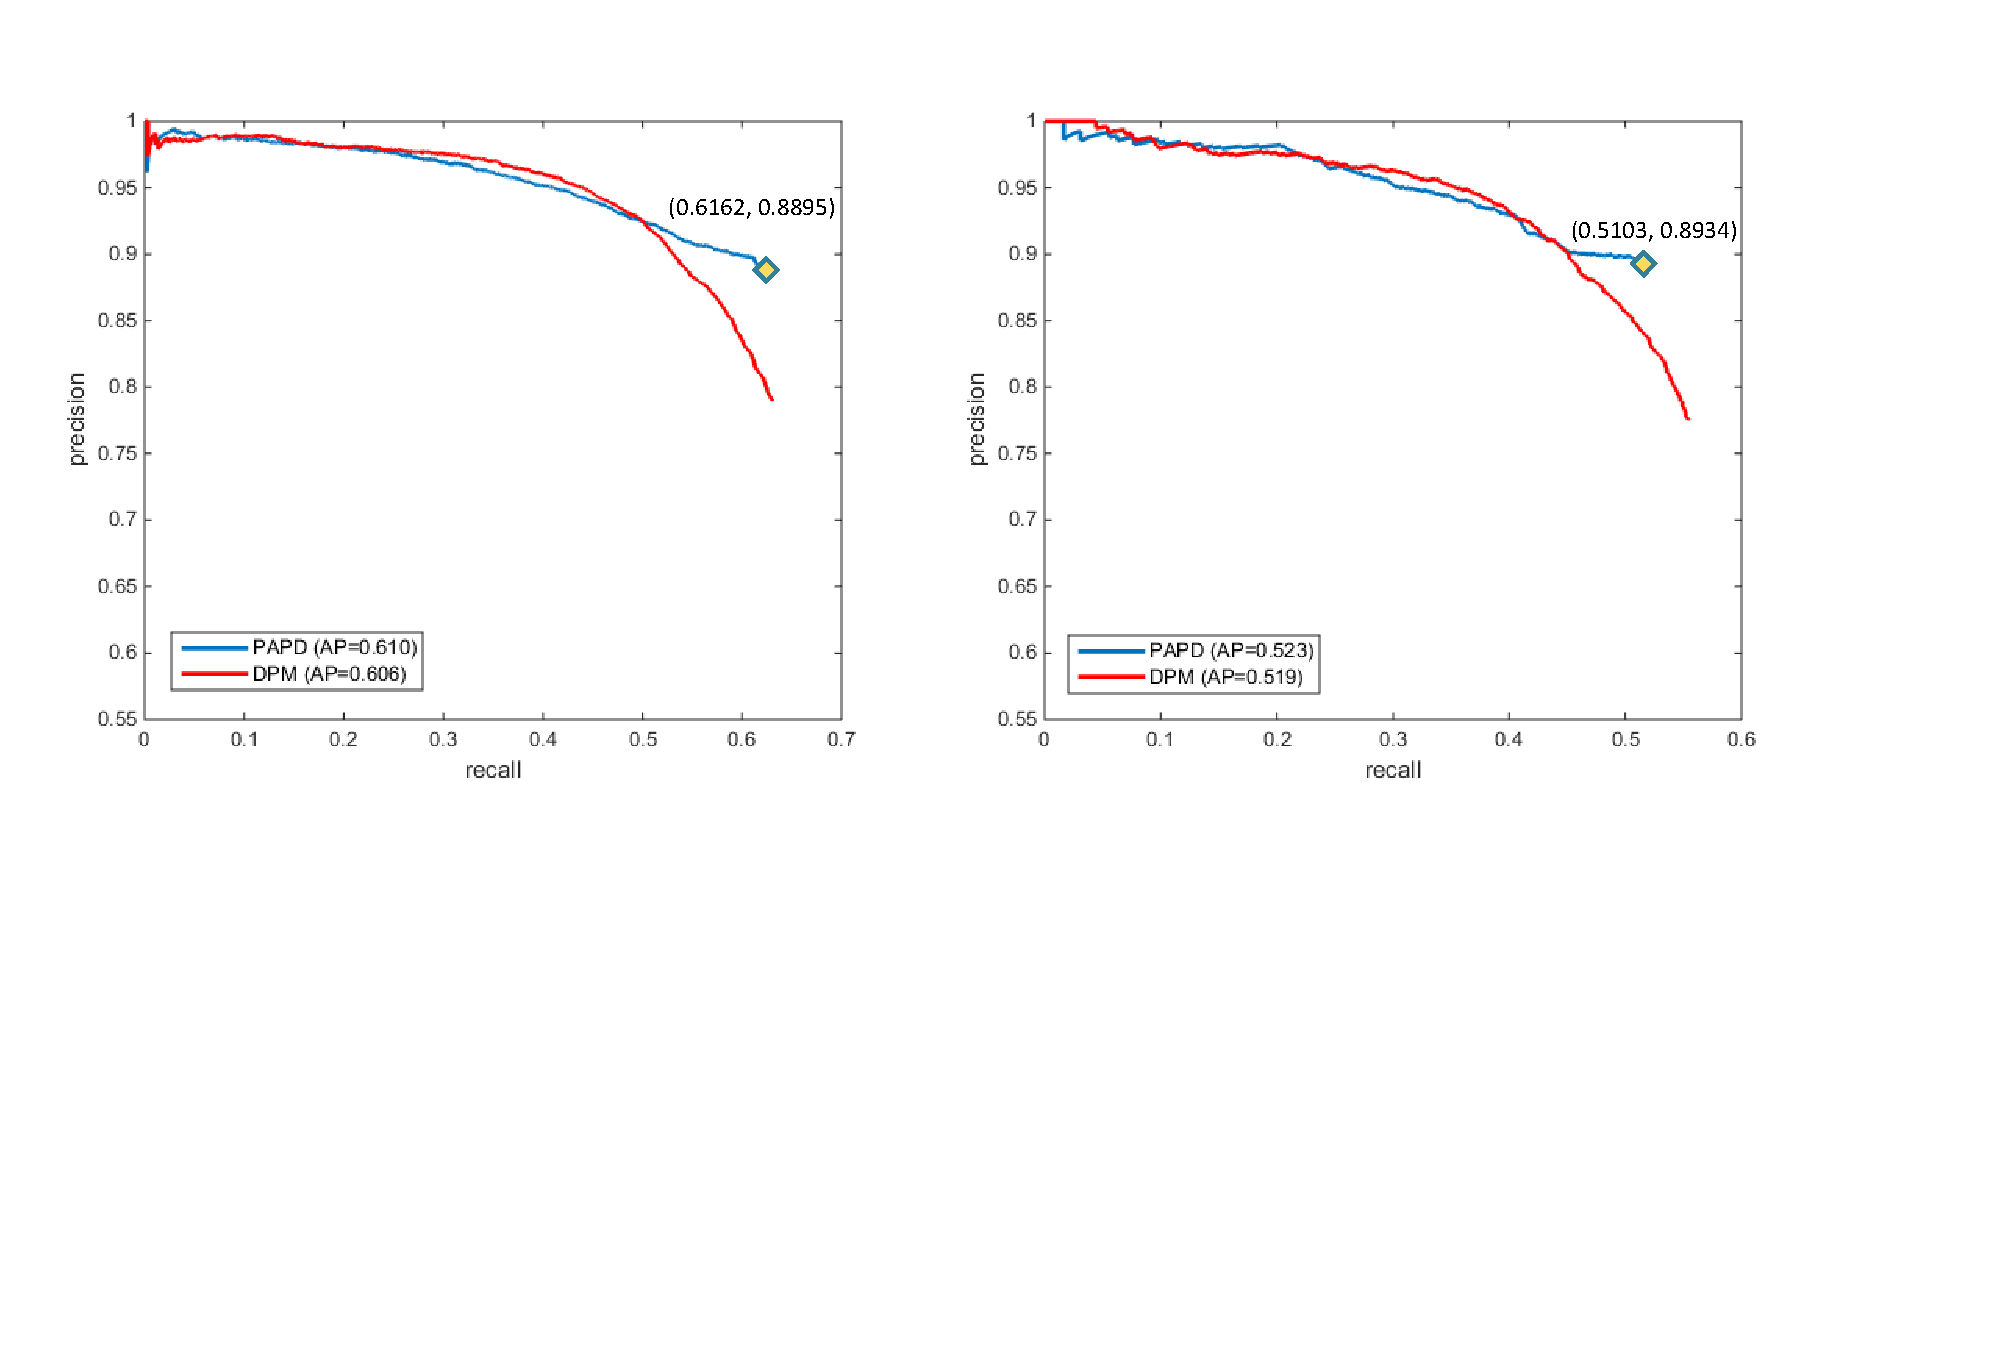
\includegraphics[width=1.0\textwidth]{../figures/ROC.pdf}
   \caption{Recall-Precision curves of PETS2009 S2.L2 (left) and S2.L3(right).}
   \label{fig:exp_roc}
\end{figure*}
\begin{figure*}
   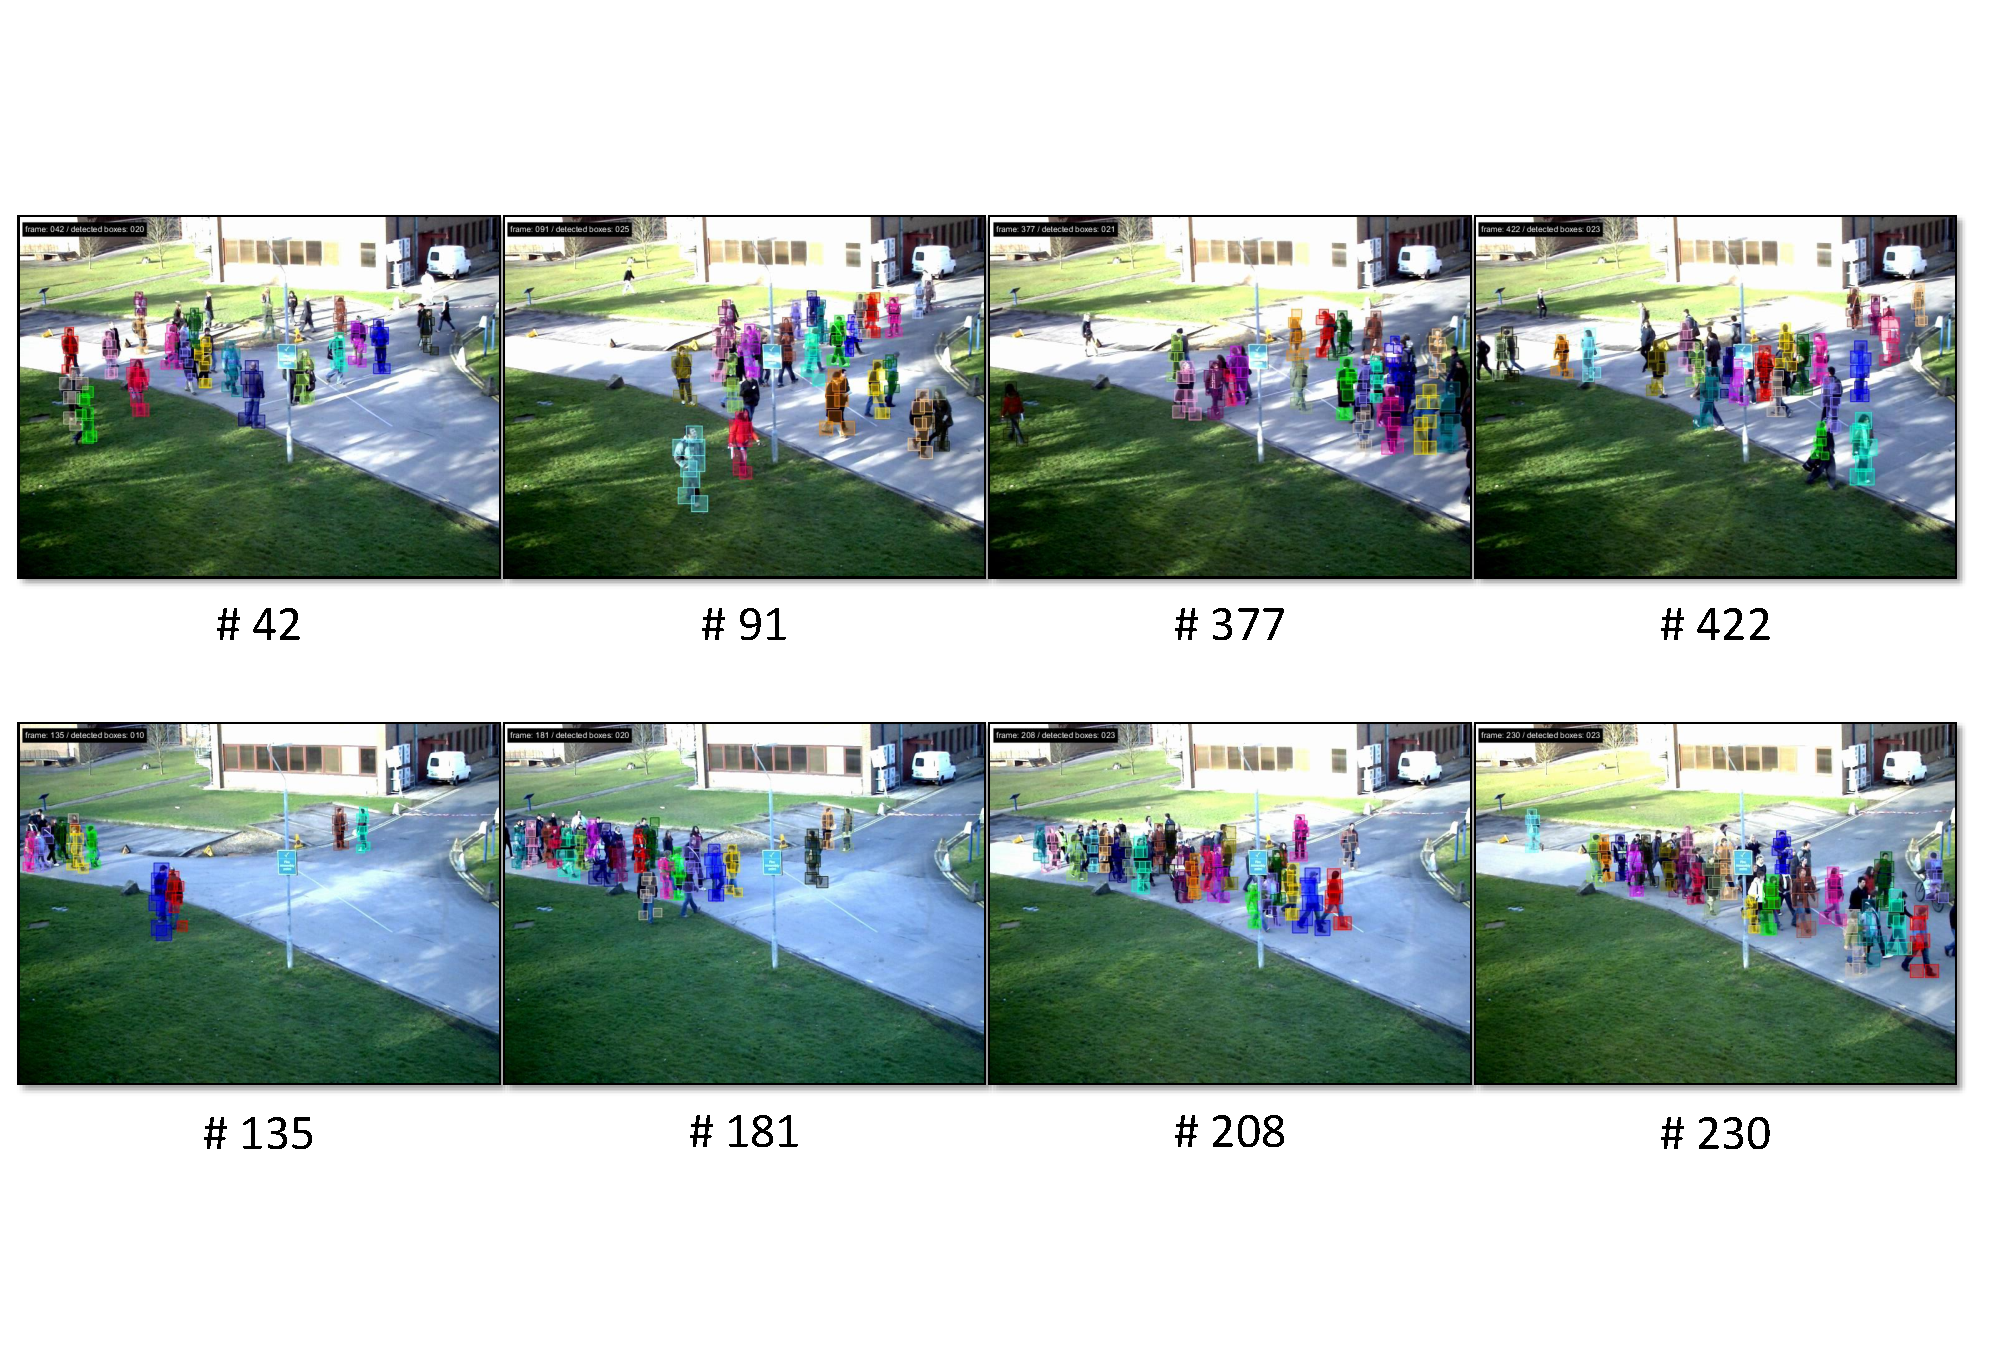
\includegraphics[width=1.0\textwidth]{../figures/experimental_result.pdf}
   \caption{Detection result of proposed method on PETS2009 S2.L2 (upper raw) and S2.L3 (lower raw).}
   \label{fig:exp_scenes}
\end{figure*}
% dataset
We evaluate the performance of the proposed method in PETS2009\footnote{http://www.cvg.rdg.ac.uk/PETS2009/a.html} dataset, the widely used public benchmarks in multi-pedestrian detection and tracking.
We select S2.L2 and S2.L3 each the set of medium and high density crowd scenes.
We use the annotations distributed by Anton Milan\footnote{http://www.milanton.de/data.html\#gt} for our evaluations.
We draw recall-precision curves with the PASCAL VOC criterion~\cite{everingham2010pascal} and select AP(average-Precision) as the comparison measure.
% training set
For the input part detector and the SVM in the pruning of part combinations, we use INRIA training dataset in~\cite{dalal2005histograms}.
% 우리는 part detector로 DPM [주석] with modified HOG feature [주석]를 사용하였으며, 이는 INRIA trainint dataset [주석]에서 학습하였다.
% Part combination validation을 위한 SVM 역시 INRIA trainint dataset에서 학습하였다.
We do not use any of scene adaptations or additional prior informations.
% 그 외에는 scene adaptation이나 prior 정보 추출을 위한 어떠한 학습도 수행하지 않았다.
In our implementation, we use $\theta_h = 0.8, \theta_c = 0.3, \theta_d = 6, \lambda_1 = 1$ and $\lambda_2 = $ in the entire experiments.

We mainly compare with DPM, the mose widely used algorithm in the recent years.
Although Yan $et al.$ provides the evaluation results of their method in \cite{yan2012multi}, it is impossible to make a fair comparison between their method and our method since they used crucial prior informations in their experiment.
Futhermore, they have not provided their annotations.

Fig.~\ref{fig:exp_roc} shows the recall-precision curves of experiments on the benchmark. 
The proposed method is refered as PAPD.
The diamon shapes colored by yellow and numbers written above the shapes represent recall-precision values of the optimal assocation hypothesis.
As shown in the figure, the precisions with the high recall are notably improved.
However, the improvements in AP on both S2.L2 and S2.L3 are negligible.
The goal of the proposed is not to generate precise scores of part detections but to find the best association hypothesis, we use the detection score of part combinations which is identical to the score in DPM.
Thus, 

Fig.~\ref{fig:exp_scenes} shows the qualitative results of the proposed method. As depicted in the figure, the proposed method provides fine appearances of each pedestrian.

% 비교 알고리즘들
% 우리는 제안하는 방법의 성능을 mainly compare with DPM 하였다.
% 이는, 같은 part detection결과를 입력으로 사용하였을 때, 단일 보행자를 대상으로 모델링한 DPM의 star-model에 비해, 우리의 part association이 얼마나 성능을 높이는지를 알아보기 위함이다.
% 이 외에도 ACF[주석]와 Crosstalk[주석]에 대해서도 성능을 비교하였다.
% 또한 [modeling mutual visibility]에 대해서는 해당 논문에 depict된 도표를 기준으로 비교하기 위해, 제안하는 알고리즘의 S2L2와 S2L3의 결과를 병합하여 표시하였다.
% 비록 crowd scene을 위해 제안된 또다른 방법인 [GV]가 존재하나, 해당 알고리즘은 탐지하고자 하는 scene보다 더 sevear하게 crowd한 scene들을 training set으로 요구하기 때문에 실효성이 없다고 판단하였을 뿐 아니라, annotation도 공개되어 있지 않아 비교에서 제외하였다.

% \paragraph{Quantitative analysis:}
% 우리 알고리즘의 성능이 ...\% 올랐고 등등등...
% 어떤 상황에서 더 좋고...
% recall을 증가시킴에도 precision이 많이 떨어지지 않는다.

% \paragraph{Qualitative analysis:}
% 본 알고리즘은 figure에서 보듯이 머리만 나온것도 잘 분간해 낸다...
% 허나 figure에서 보듯이 한 사람을 두 사람으로 나눠서 찾기도 한다.
% 이는 해결해야 할 문제이다.
%==============================================================================



%%%%%%%%%%%%%%%%%%%%%%%%%%%%%%%%%%%%%%%%%%%%%%%%%%%%%%%%%%%%%%%%%%%%%%%%%%%%%%%
% CONCLUSION
%%%%%%%%%%%%%%%%%%%%%%%%%%%%%%%%%%%%%%%%%%%%%%%%%%%%%%%%%%%%%%%%%%%%%%%%%%%%%%%
\section{Conclusion}
\label{sec:conclusion}
In this paper, we propose a novel pedestrian detection method which consider an overall occlusion in the target image.
Experiments on the public benchmark validate the robust performance of the proposed method.

%==============================================================================



% %%%%%%%%%%%%%%%%%%%%%%%%%%%%%%%%%%%%%%%%%%%%%%%%%%%%%%%%%%%%%%%%%%%%%%%%%%%%%%%
% % ACKNOWLEDGEMENTS
% %%%%%%%%%%%%%%%%%%%%%%%%%%%%%%%%%%%%%%%%%%%%%%%%%%%%%%%%%%%%%%%%%%%%%%%%%%%%%%%
% \begin{acknowledgements}
% This work was supported by the IT R\&D program of MOTIE/KEIT. [10041610, The development of automatic user information(identification, behavior, location) extraction and recognition technology based on perception sensor network(PSN) under real environment for intelligent robot]
% \end{acknowledgements}
% %==============================================================================



%%%%%%%%%%%%%%%%%%%%%%%%%%%%%%%%%%%%%%%%%%%%%%%%%%%%%%%%%%%%%%%%%%%%%%%%%%%%%%%
% REFERENCES
%%%%%%%%%%%%%%%%%%%%%%%%%%%%%%%%%%%%%%%%%%%%%%%%%%%%%%%%%%%%%%%%%%%%%%%%%%%%%%%
{\small
\bibliographystyle{splncs}
\bibliography{eccv2016submission_PAPD}
}
%==============================================================================

\section{Paper formatting}

\subsection{Language}

All manuscripts must be in English.

\subsection{Paper length}
Papers submitted for review should be complete. 
The length should match that intended for final publication. 
Papers accepted for the conference will be allocated 14 pages (plus references) in the proceedings. 
Note that the allocated 14 pages do not include the references. The reason for this policy
is that we do not want authors to omit references for sake of space limitations.

Papers with more than 14 pages (excluding references) will be rejected without review.
This includes papers where the margins and
formatting are deemed to have been significantly altered from those
laid down by this style guide.  The reason such papers will not be
reviewed is that there is no provision for supervised revisions of
manuscripts. The reviewing process cannot determine the suitability of
the paper for presentation in 14 pages if it is reviewed in 16.

\subsection{Paper ID}

It is imperative that the paper ID is mentioned on each page of the manuscript.
The paper ID is a number automatically assigned to your submission when 
registering your paper submission on CMT.


\subsection{Line numbering}

All lines should be numbered, as in this example document.  This makes
reviewing more efficient, because reviewers can refer to a line on a
page.  If you are preparing a document using a non-\LaTeX\
document preparation system, please arrange for an equivalent line numbering.



\subsection{Mathematics}

Please number all of your sections and displayed equations.  Again,
this makes reviewing more efficient, because reviewers can refer to a
line on a page.  Also, it is important for readers to be able to refer
to any particular equation.  Just because you didn't refer to it in
the text doesn't mean some future reader might not need to refer to
it.  It is cumbersome to have to use circumlocutions like ``the
equation second from the top of page 3 column 1''.  (Note that the
line numbering will not be present in the final copy, so is not an
alternative to equation numbers).  Some authors might benefit from
reading Mermin's description of how to write mathematic.

\section{Blind review}
\label{sec:blind}

Many authors misunderstand the concept of anonymizing for blind
review.  Blind review does not mean that one must remove
citations to one's own work. In fact it is often impossible to
review a paper unless the previous citations are known and
available.

Blind review means that you do not use the words ``my'' or ``our''
when citing previous work.  That is all.  (But see below for
technical reports).

Saying ``this builds on the work of Lucy Smith [1]'' does not say
that you are Lucy Smith, it says that you are building on her
work.  If you are Smith and Jones, do not say ``as we show in
[7]'', say ``as Smith and Jones show in [7]'' and at the end of the
paper, include reference 7 as you would any other cited work.

An example of a bad paper:
\begin{quote}
\begin{center}
    An analysis of the frobnicatable foo filter.
\end{center}

   In this paper we present a performance analysis of our
   previous paper [1], and show it to be inferior to all
   previously known methods.  Why the previous paper was
   accepted without this analysis is beyond me.

   [1] Removed for blind review
\end{quote}


An example of an excellent paper:

\begin{quote}
\begin{center}
     An analysis of the frobnicatable foo filter.
\end{center}

   In this paper we present a performance analysis of the
   paper of Smith [1], and show it to be inferior to
   all previously known methods.  Why the previous paper
   was accepted without this analysis is beyond me.

   [1] Smith, L. and Jones, C. ``The frobnicatable foo
   filter, a fundamental contribution to human knowledge''.
   Nature 381(12), 1-213.
\end{quote}

If you are making a submission to another conference at the same
time, which covers similar or overlapping material, you may need
to refer to that submission in order to explain the differences,
just as you would if you had previously published related work. In
such cases, include the anonymized parallel
submission~\cite{Authors14} as additional material and cite it as
\begin{quote}
1. Authors. ``The frobnicatable foo filter'', BMVC 2014 Submission
ID 324, Supplied as additional material {\tt bmvc14.pdf}.
\end{quote}

Finally, you may feel you need to tell the reader that more
details can be found elsewhere, and refer them to a technical
report.  For conference submissions, the paper must stand on its
own, and not {\em require} the reviewer to go to a techreport for
further details.  Thus, you may say in the body of the paper
``further details may be found in~\cite{Authors14b}''.  Then
submit the techreport as additional material. Again, you may not
assume the reviewers will read this material.

Sometimes your paper is about a problem which you tested using a tool which
is widely known to be restricted to a single institution.  For example,
let's say it's 1969, you have solved a key problem on the Apollo lander,
and you believe that the ECCV audience would like to hear about your
solution.  The work is a development of your celebrated 1968 paper entitled
``Zero-g frobnication: How being the only people in the world with access to
the Apollo lander source code makes us a wow at parties'', by Zeus.

You can handle this paper like any other.  Don't write ``We show how to
improve our previous work [Anonymous, 1968].  This time we tested the
algorithm on a lunar lander [name of lander removed for blind review]''.
That would be silly, and would immediately identify the authors. Instead
write the following:
\begin{quotation}
\noindent
   We describe a system for zero-g frobnication.  This
   system is new because it handles the following cases:
   A, B.  Previous systems [Zeus et al. 1968] didn't
   handle case B properly.  Ours handles it by including
   a foo term in the bar integral.

   ...

   The proposed system was integrated with the Apollo
   lunar lander, and went all the way to the moon, don't
   you know.  It displayed the following behaviours
   which show how well we solved cases A and B: ...
\end{quotation}
As you can see, the above text follows standard scientific convention,
reads better than the first version, and does not explicitly name you as
the authors.  A reviewer might think it likely that the new paper was
written by Zeus, but cannot make any decision based on that guess.
He or she would have to be sure that no other authors could have been
contracted to solve problem B. \\

For sake of anonymity, it's recommended to omit acknowledgements
in your review copy. They can be added later when you prepare the final copy.



\section{Manuscript Preparation}

This is an edited version of Springer LNCS instructions adapted
for ECCV 2016 first paper submission.
You are strongly encouraged to use \LaTeX2$_\varepsilon$ for the
preparation of your
camera-ready manuscript together with the corresponding Springer
class file \verb+llncs.cls+.

We would like to stress that the class/style files and the template
should not be manipulated and that the guidelines regarding font sizes
and format should be adhered to. This is to ensure that the end product
is as homogeneous as possible.

\subsection{Printing Area}
The printing area is $122  \; \mbox{mm} \times 193 \;
\mbox{mm}$.
The text should be justified to occupy the full line width,
so that the right margin is not ragged, with words hyphenated as
appropriate. Please fill pages so that the length of the text
is no less than 180~mm.

\subsection{Layout, Typeface, Font Sizes, and Numbering}
Use 10-point type for the name(s) of the author(s) and 9-point type for
the address(es) and the abstract. For the main text, please use 10-point
type and single-line spacing.
We recommend using Computer Modern Roman (CM) fonts, Times, or one
of the similar typefaces widely used in photo-typesetting.
(In these typefaces the letters have serifs, i.e., short endstrokes at
the head and the foot of letters.)
Italic type may be used to emphasize words in running text. Bold
type and underlining should be avoided.
With these sizes, the interline distance should be set so that some 45
lines occur on a full-text page.

\subsubsection{Headings.}

Headings should be capitalized
(i.e., nouns, verbs, and all other words
except articles, prepositions, and conjunctions should be set with an
initial capital) and should,
with the exception of the title, be aligned to the left.
Words joined by a hyphen are subject to a special rule. If the first
word can stand alone, the second word should be capitalized.
The font sizes
are given in Table~\ref{table:headings}.
\setlength{\tabcolsep}{4pt}
\begin{table}
\begin{center}
\caption{Font sizes of headings. Table captions should always be
positioned {\it above} the tables. The final sentence of a table
caption should end without a full stop}
\label{table:headings}
\begin{tabular}{lll}
\hline\noalign{\smallskip}
Heading level & Example & Font size and style\\
\noalign{\smallskip}
\hline
\noalign{\smallskip}
Title (centered)  & {\Large \bf Lecture Notes \dots} & 14 point, bold\\
1st-level heading & {\large \bf 1 Introduction} & 12 point, bold\\
2nd-level heading & {\bf 2.1 Printing Area} & 10 point, bold\\
3rd-level heading & {\bf Headings.} Text follows \dots & 10 point, bold
\\
4th-level heading & {\it Remark.} Text follows \dots & 10 point,
italic\\
\hline
\end{tabular}
\end{center}
\end{table}
\setlength{\tabcolsep}{1.4pt}

Here are
some examples of headings: ``Criteria to Disprove Context-Freeness of
Collage Languages'', ``On Correcting the Intrusion of Tracing
Non-deterministic Programs by Software'', ``A User-Friendly and
Extendable Data Distribution System'', ``Multi-flip Networks:
Parallelizing GenSAT'', ``Self-determinations of Man''.

\subsubsection{Lemmas, Propositions, and Theorems.}

The numbers accorded to lemmas, propositions, and theorems etc. should
appear in consecutive order, starting with the number 1, and not, for
example, with the number 11.

\subsection{Figures and Photographs}
\label{sect:figures}

Please produce your figures electronically and integrate
them into your text file. For \LaTeX\ users we recommend using package
\verb+graphicx+ or the style files \verb+psfig+ or \verb+epsf+.

Check that in line drawings, lines are not
interrupted and have constant width. Grids and details within the
figures must be clearly readable and may not be written one on top of
the other. Line drawings should have a resolution of at least 800 dpi
(preferably 1200 dpi).
For digital halftones 300 dpi is usually sufficient.
The lettering in figures should have a height of 2~mm (10-point type).
Figures should be scaled up or down accordingly.
Please do not use any absolute coordinates in figures.

Figures should be numbered and should have a caption which should
always be positioned {\it under} the figures, in contrast to the caption
belonging to a table, which should always appear {\it above} the table.
Please center the captions between the margins and set them in
9-point type
(Fig.~\ref{fig:example} shows an example).
The distance between text and figure should be about 8~mm, the
distance between figure and caption about 5~mm.
\begin{figure}
\centering
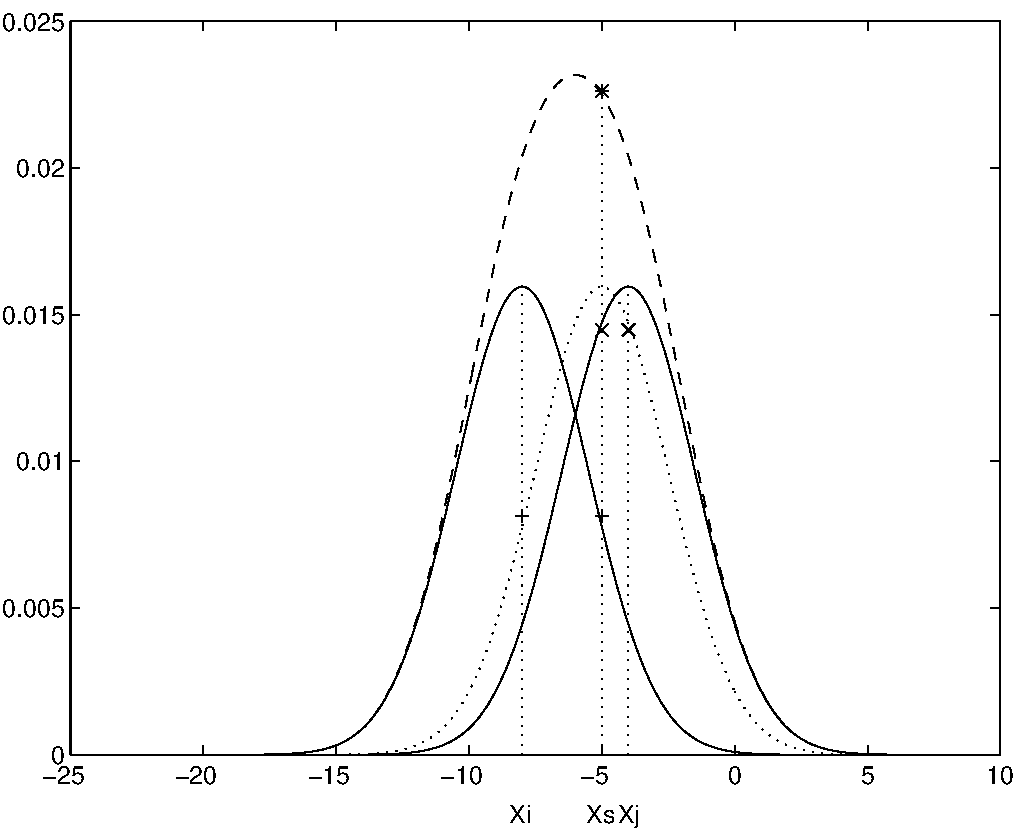
\includegraphics[height=6.5cm]{eijkel2}
\caption{One kernel at $x_s$ ({\it dotted kernel}) or two kernels at
$x_i$ and $x_j$ ({\it left and right}) lead to the same summed estimate
at $x_s$. This shows a figure consisting of different types of
lines. Elements of the figure described in the caption should be set in
italics,
in parentheses, as shown in this sample caption. The last
sentence of a figure caption should generally end without a full stop}
\label{fig:example}
\end{figure}

If possible (e.g. if you use \LaTeX) please define figures as floating
objects. \LaTeX\ users, please avoid using the location
parameter ``h'' for ``here''. If you have to insert a pagebreak before a
figure, please ensure that the previous page is completely filled.


\subsection{Formulas}

Displayed equations or formulas are centered and set on a separate
line (with an extra line or halfline space above and below). Displayed
expressions should be numbered for reference. The numbers should be
consecutive within the contribution,
with numbers enclosed in parentheses and set on the right margin.
For example,
\begin{align}
  \psi (u) & = \int_{0}^{T} \left[\frac{1}{2}
  \left(\Lambda_{0}^{-1} u,u\right) + N^{\ast} (-u)\right] dt \; \\
& = 0 ?
\end{align}

Please punctuate a displayed equation in the same way as ordinary
text but with a small space before the end punctuation.

\subsection{Footnotes}

The superscript numeral used to refer to a footnote appears in the text
either directly after the word to be discussed or, in relation to a
phrase or a sentence, following the punctuation sign (comma,
semicolon, or full stop). Footnotes should appear at the bottom of
the
normal text area, with a line of about 2~cm in \TeX\ and about 5~cm in
Word set
immediately above them.\footnote{The footnote numeral is set flush left
and the text follows with the usual word spacing. Second and subsequent
lines are indented. Footnotes should end with a full stop.}


\subsection{Program Code}

Program listings or program commands in the text are normally set in
typewriter font, e.g., CMTT10 or Courier.

\noindent
{\it Example of a Computer Program}
\begin{verbatim}
program Inflation (Output)
  {Assuming annual inflation rates of 7%, 8%, and 10%,...
   years};
   const
     MaxYears = 10;
   var
     Year: 0..MaxYears;
     Factor1, Factor2, Factor3: Real;
   begin
     Year := 0;
     Factor1 := 1.0; Factor2 := 1.0; Factor3 := 1.0;
     WriteLn('Year  7% 8% 10%'); WriteLn;
     repeat
       Year := Year + 1;
       Factor1 := Factor1 * 1.07;
       Factor2 := Factor2 * 1.08;
       Factor3 := Factor3 * 1.10;
       WriteLn(Year:5,Factor1:7:3,Factor2:7:3,Factor3:7:3)
     until Year = MaxYears
end.
\end{verbatim}
%
\noindent
{\small (Example from Jensen K., Wirth N. (1991) Pascal user manual and
report. Springer, New York)}



\subsection{Citations}

The list of references is headed ``References" and is not assigned a
number
in the decimal system of headings. The list should be set in small print
and placed at the end of your contribution, in front of the appendix,
if one exists.
Please do not insert a pagebreak before the list of references if the
page is not completely filled.
An example is given at the
end of this information sheet. For citations in the text please use
square brackets and consecutive numbers: \cite{Alpher02},
\cite{Alpher03}, \cite{Alpher04} \dots

\section{Conclusions}

The paper ends with a conclusion. 


\clearpage\mbox{}Page \thepage\ of the manuscript.
\clearpage\mbox{}Page \thepage\ of the manuscript.
\clearpage\mbox{}Page \thepage\ of the manuscript.
\clearpage\mbox{}Page \thepage\ of the manuscript.
\clearpage\mbox{}Page \thepage\ of the manuscript.
\clearpage\mbox{}Page \thepage\ of the manuscript.
\clearpage\mbox{}Page \thepage\ of the manuscript.
This is the last page of the manuscript.
\par\vfill\par
Now we have reached the maximum size of the ECCV 2016 submission (excluding references).
References should start immediately after the main text, but can continue on p.15 if needed.

\clearpage

\end{document}
